\documentclass[a4paper,twoside,12pt,chapterprefix=false]{scrbook}

\usepackage{amsmath,amssymb,amsthm}
\usepackage[footnotesize,sl,SL,hang,tight]{subfigure}  % helpful package for aligning figures next to each other
\usepackage{longtable} % tables over several pages
\usepackage[font={small,sl},hang,labelfont=bf]{caption} % configure captions
%\usepackage{captcont} % continue sufigures over several pages
\usepackage{booktabs} % publication quality tables for LaTeX
%\usepackage{showkeys} % shows the labels above the references for easier development

\ifpdfoutput{%
	\usepackage[pdftex]{graphicx}
	\usepackage[]{pdfpages} %for including full pdf pages
}{%
	\usepackage{graphicx}
}
\usepackage{rotating} % rotate figures

\usepackage{scrlayer-scrpage}
\KOMAoptions{headinclude}

% Font packages:
\usepackage{times}
\usepackage{helvet}   % sets sans serif font
\usepackage[T1]{fontenc}

%PDF hyperref config
\ifpdfoutput{%
	\usepackage[pdftex,
		bookmarks,
		bookmarksopen=true,
		bookmarksnumbered=true,
		pdfauthor={My Name},
		pdftitle={Thesis Title},
		colorlinks,
		linkcolor=black,
		citecolor=black,
		filecolor=black,
		urlcolor=black,
		anchorcolor=black,
		menucolor=black,
		breaklinks=true,
		pageanchor=true,
		plainpages=false,
		pdfpagelabels=true]{hyperref}
}{}

\ifpdfoutput{%
	\pdfcompresslevel=9
	\pdfoutput=1
	\DeclareGraphicsExtensions{.pdf,.png}
}{}

\bibliographystyle{alpha}

% Uncomment the chapter / section you are working on.
%
%\includeonly{figures}
%\includeonly{tables}
%\includeonly{data-analysis}
%\includeonly{conclusion}
%\includeonly{apx-sample-appendix}

%\pagestyle{useheadings}

% A4
%
\topmargin -0.5in
\textheight 9.3in
\textwidth 6.3in
\oddsidemargin 0.18in
\evensidemargin -0.22in
\parskip 0.1in
\parindent 0in

\renewcommand{\arraystretch}{1.5}
\renewcommand{\baselinestretch}{1}

% commands
\newcommand{\Adjoint}{\mbox{\rm Adj}}
\newcommand{\Area}{\mbox{\rm Area}}
\newcommand{\ACos}{{\mbox{\rm Cos}^{-1}}}
\newcommand{\ASin}{{\mbox{\rm Sin}^{-1}}}
\newcommand{\ATan}{{\mbox{\rm atan2}}}
\newcommand{\Code}[1]{{\tt #1}}
\newcommand{\Complex}{\mbox{\bf C}}
\newcommand{\Cross}{{\mbox{\rm Cross}}}
\newcommand{\Mydddot}[1]{\mbox{\shortstack{$.$\hspace*{-1pt}$.$\hspace*{-1pt}$.$\\$#1$}}}
\newcommand{\Degree}{\mbox{\rm degree}}
\newcommand{\Diag}{\mbox{\rm Diag}}
\newcommand{\Dim}{\mbox{\rm dim}}
\newcommand{\Dist}{\mbox{\rm Distance}}
\newcommand{\IntTwo}{\int\!\!\int}
\newcommand{\IntThree}{\int\!\!\int\! \!\int}
\newcommand{\Kernel}{\mbox{\rm kernel}}
\newcommand{\Kross}{\mbox{\rm Kross}}
\newcommand{\Grad}{\nabla}
\newcommand{\Perp}{\mbox{\rm Perp}}
\newcommand{\Point}[1]{{\cal #1}}
\newcommand{\Rank}{\mbox{\rm rank}}
\newcommand{\Range}{\mbox{\rm range}}
\newcommand{\Real}{{\mbox{\rm I}\hspace*{-2pt}\mbox{\rm R}}}
\newcommand{\RealSbt}{{\mbox{\rm\scriptsize I}\hspace*{-2pt}\mbox{\rm\scriptsize R}}}
\newcommand{\Res}{\mbox{\rm resultant}}
\newcommand{\Sbt}[1]{{\mbox{\rm\scriptsize #1}}}
\newcommand{\MySign}{\mbox{\rm Sign}}
\newcommand{\SignSBT}{\mbox{\rm\scriptsize Sign}}
\newcommand{\Skew}{\mbox{\rm Skew}}
\newcommand{\Span}{\mbox{\rm Span}}
\newcommand{\SqrDist}{\mbox{\rm Distance$^2$}}
\newcommand{\Trace}{\mbox{\rm Trace}}
\newcommand{\TRN}{{\mbox{\rm\scriptsize T}}}
\newcommand{\Vector}[1]{\mbox{\bf #1}}
\newcommand{\VectorM}[1]{\mbox{\boldmath $#1$}}
\newcommand{\Volume}{\mbox{\rm Volume}}

\newcommand{\IVec}{\mbox{\boldmath $\imath$}}
\newcommand{\JVec}{\mbox{\boldmath $\jmath$}}
\newcommand{\KVec}{\mbox{\boldmath $k$}}
\newcommand{\LVec}{\mbox{\boldmath $\ell$}}
\newcommand{\RMat}{{\cal R}}
\newcommand{\QMat}{{\cal Q}}
\newcommand{\QCMat}{\overline{\cal Q}}

\newcommand{\Lerp}{\mbox{\rm lerp}}
\newcommand{\Slerp}{\mbox{\rm slerp}}
\newcommand{\Quad}{\mbox{\rm quad}}
\newcommand{\Squad}{\mbox{\rm squad}}

\newcommand{\subsubsubsection}[1]{{\sc #1}}

\newcommand{\ODer}[2]{\frac{d #1}{d #2}}
\newcommand{\ODerT}[2]{\frac{d^2 #1}{d {#2}^2}}
\newcommand{\ODerM}[3]{\frac{d #1}{d #2 \, d #3}}
\newcommand{\PDer}[2]{\frac{\partial #1}{\partial #2}}
\newcommand{\PDerT}[2]{\frac{\partial^2 #1}{\partial {#2}^2}}
\newcommand{\PDerM}[3]{\frac{\partial^2 #1}{\partial #2 \, \partial #3}}

% mass density symbol
\newcommand{\Den}{\delta}

% environments
\newenvironment{BArray}[1]{\left\{ \begin{array}{#1}}{\end{array} \right\}}
\newenvironment{Combin}{\left( \begin{array}{c}}{\end{array} \right)}
\newenvironment{Matrix}[1]{\left[ \begin{array}{#1}}{\end{array} \right]}

% "Figure" environment
\newtheorem{localFigure}{Figure}[chapter]
\newenvironment{Figure}[1]{
  \begin{center}
  \begin{minipage}{6in}
  \par\noindent\hspace*{0pt}\hrulefill
  
  \begin{localFigure} \label{#1}
}{
  \end{localFigure}
  \par\noindent\hspace*{0pt}\hrulefill
  \end{minipage}
  \end{center}
}

% "Table" environment
\newtheorem{localTable}{Table}[chapter]
\newenvironment{Table}[1]{
  \begin{center}
  \begin{minipage}{6in}
  
  \begin{localTable} \label{#1}
}{
  \end{localTable}
  \end{minipage}
  \end{center}
}

% "CDROM" environment for source code on disk
%\newenvironment{CDROM}[1]{
%  \label{#1} 
%    \includegraphics{cdrom.png} \hspace*{0.1in}{\tt PointShop3D}. \rm
%}{
%  $\bowtie$
%}

% TO DO search symbol
\newcommand{\TODO}{\mbox{\large\bf TO DO}}
\newcommand{\REFR}{\mbox{\large\bf REFR}}

%  Terminates current page and paragraph, makes sure next page starts on
%  an odd-number, and generates a completely blank page, without page markers,
%  if necessary.
\newcommand{\clearemptydoublepage}{\newpage{\pagestyle{empty}\cleardoublepage}}

%%% Shoemake's commands
\DeclareMathOperator{\prp}{\text{\scshape perp}}
\DeclareMathOperator{\rot}{rot}
\DeclareMathOperator{\N}{N}
\providecommand{\vmag}[1]{\lVert#1\rVert}
\providecommand{\mutate}[1]{\overleftarrow{#1}}
\providecommand{\T}[1]{{#1}^{\mathrm T}}
\newcommand{\cross}{\times}
\newcommand{\by}{\times}
\newcommand{\vect}[1]{\mathbf{#1}}
\newcommand{\mat}[1]{\mathbf{#1}} % or not
%\newcommand{\quat}[1]{\mathbf{#1}}
\newcommand{\quat}[1]{\ensuremath{\mathbf{\dot{#1}}}}
\newcommand{\vV}{\vect{v}}
\newcommand{\vU}{\vect{u}}
\newcommand{\vE}{\vect{e}}
\newcommand{\vUh}{\hat{\vect{u}}}
\newcommand{\mQ}{\mat{Q}}
\newcommand{\mR}{\mat{R}}
\newcommand{\mM}{\mat{M}}
\newcommand{\mA}{\mat{A}}
\newcommand{\mB}{\mat{B}}
\newcommand{\mI}{\mat{I}}
\newcommand{\mJ}{\mat{J}}
\newcommand{\mX}{\mat{X}}
\newcommand{\mY}{\mat{Y}}
\newcommand{\mZ}{\mat{Z}}
\newcommand{\qo}{\quat{1}}
\newcommand{\qi}{\quat{i}}
\newcommand{\qj}{\quat{j}}
\newcommand{\qk}{\quat{k}}
\newcommand{\xh}{{x}}
\newcommand{\yh}{{y}}
\newcommand{\zh}{{z}}
\newcommand{\ch}{c}
\newcommand{\sh}{s}
\newcommand{\gt}{\theta}


%%
%%  include additional packages
%% 
% \usepackage{tikz}
% \usepackage{pgfplots}


\begin{document}

%% Define leading chapter pages
%
%\addtokomafont{chapter}{\setlength{\parskip}{190pt}}   % SEVERE HACK to keep spacing to chapter art work
\renewcommand*{\chapterheadstartvskip}{\vspace*{215pt}}  % different hack to keep spacing to chapter artwork
%\addtokomafont{chapter}{\rmfamily}        % remove this if you prefer sans-serif section titles
%\addtokomafont{section}{\rmfamily}        % remove this if you prefer sans-serif section titles
%\addtokomafont{subsection}{\rmfamily}     % remove this if you prefer sans-serif section titles
%\addtokomafont{subsubsection}{\rmfamily}  % remove this if you prefer sans-serif section titles
%\addtokomafont{paragraph}{\rmfamily}      % replace by \sffamily if you prefer sans-serif para titles
\addtokomafont{paragraph}{\sffamily}

\def\mychpstyleintl{%
{\noindent\setlength{\tabcolsep}{0pt}\setlength{\arrayrulewidth}{2pt}%
\begin{tabular}{c}
\\[100pt]
\begin{tabular}{lr}
\begin{tabular}{p{0.6\linewidth}}
\\
\end{tabular}
&
\begin{tabular}{p{0.4\linewidth}}
\rightline{{%
\sffamily%
\fontseries{bx}%
\fontshape{n}%
\fontsize{100}{120}%choose baselineskip to be 1.2 times font size
\selectfont
\thechapter}}
\end{tabular}
\end{tabular}\\[300pt]
\end{tabular}
}}

\newpagestyle{mychapterpagestyle}{{\protect\mychpstyleintl}{\protect\mychpstyleintl}}{}
\newpagestyle{myappendixpagestyle}{{\protect\mychpstyleintl}{\protect\mychpstyleintl}}{}
%%

%% macros e.g.
\newcommand{\mfytext}[0]{my fancy text}

%refs
\newcommand{\chpref}[1]{Chapter \ref{#1}}
\newcommand{\secref}[1]{Section \ref{#1}}
%\newcommand{\equref}[1]{Equation \ref{#1}} %better use builtin \eqref{}
\newcommand{\figref}[1]{Figure \ref{#1}}
\newcommand{\tabref}[1]{Table \ref{#1}}
\newcommand{\apxref}[1]{Appendix \ref{#1}}
%%

\hypersetup{pageanchor=false} % disabling anchors for title page to avoid warning

%% Replace this by your own design of a title page
%
%\title{Thesis Title}
%\author{My Name}
%\date{September 2042}
%\maketitle
%\clearemptydoublepage
% --- selfmade version ----
\begin{titlepage}
	\topmargin 1.0cm
	\oddsidemargin 0.0cm
	\evensidemargin 0.0cm
	%\textwidth 6.5in
	\centering
	\Huge
	\vspace{3.0cm}
	\textbf{\textsf{Thesis Title}} \\[2.0cm]
	%\includegraphics*[width=0.4\textwidth]{figures/titlefigure} \\[4.0cm]
	\vspace{5.0cm}
	\sffamily
	\Large
	Francesca Marsicano
	\\[0.8cm]
	\large
	Master Thesis
	\\
	March 2022
	\\[1.3cm]
	Prof. Dr. My Prof
	\vfill
	\includegraphics*[width=0.3\textwidth]{figures/ETH_logo} \hfill
	\includegraphics*[width=0.3\textwidth]{figures/CGL_logo}
	\vspace{3.4cm}
\end{titlepage}
\clearemptydoublepage
%%

\hypersetup{pageanchor=true}
\pagenumbering{roman}
\setcounter{page}{1}

\chapter*{Abstract}

Multi-person pose estimation in images and videos is an important yet challenging task with many applications.
Despite the large improvements in human pose estimation
enabled by the development of convolutional neural networks, there still exist a lot of difficult cases where even the state-of-the-art models fail to correctly localize all body joints. This motivates the need for an additional refinement step that addresses these challenging cases and can be easily applied on top of any existing method. In this work we analyze the different training protocols to extend the capabilities of he current architecture without drawing on additional ground truth labels or network stacked architecrure

%include task description here:
\cleardoublepage
%\includegraphics[viewport=3cm 0cm 20cm 27.5cm]{task_description} %better use includepdf below!
%\includepdf{task_description}
\cleardoublepage

%include acknowledgment here:
%\include{acknowledgment}

\tableofcontents
\cleardoublepage

\addcontentsline{toc}{chapter}{List of Figures}
\listoffigures
\cleardoublepage

\addcontentsline{toc}{chapter}{List of Tables}
\listoftables
\cleardoublepage

\pagenumbering{arabic}
\renewcommand*{\chapterpagestyle}{mychapterpagestyle}
\renewcommand*{\chapterformat}{} % show chapter titles only (no numbers)
% \setchapterpreamble[o]{...}  unfortunately does not move the \chapter output downwards

% ---- MAIN PART ----

% set counter to n-1:
\setcounter{chapter}{0}

\chapter{Introduction}

The goal of human pose estimation is to localize semantic keypoints of a human body. 
Recently, many methods utilize deep convolutional neural networks (CNNs) a
Conventionally, the pose refinement has been mainly performed by multi-stage architectures 


Existing methods for 3D motion capture of athletes can
be classified into those that use motion sensors and those
that use visual information only. The methods that use motion sensors can detect the accurate movement of the human
skeleton by attaching markers to the human body. However, dedicated equipment such as motion sensors are expensive and the environment for measurement is limited.
 We refine OpenPose with our newly introduce sports
dataset and a augmentation technique to improve the quality of
2D pose estimation in extreme poses.
In addition, markers must be attached on the human body,
which requires expert knowledge and may not be comfortable for the athlete. As a consequence, non-invasive techniques such as 3D pose estimation from multi-view RGB
images are preferred ( \cite{DBLP:journals/corr/abs-1907-11346}, \cite{DBLP:journals/corr/abs-1904-01324} , 
\cite{Xu_2020_CVPR}, \cite{DBLP:journals/corr/abs-2003-00529}, \cite{DBLP:journals/corr/abs-2006-07778}

[ 29],[13]). In general,
existing methods first estimate the 2D pose of the person
in each 2D image and then triangulate the 2D skeletons to
create a 3D skeleton. By doing so, a marker-less, low-cost
system that can be used anywhere can be built. In such systems, accurate and robust 2D pose estimation is critical.

If taken into account the ultimate goal of using such systems in video production the attention 

s. First, collecting accurate 3D pose annotation for RGB
images is expensive and time-consuming

The first
stage locates 2D human key-points from appearance information, while the second stage lifts the 2D joints into 3D
skeleton employing geometric information. S
% set counter to n-1:
\setcounter{chapter}{1}

\chapter{Related Work}



Sample references are~\cite{Zwicker04Perspective} and~\cite{Altman89QuaternionScandal}.

\section{Supervised learning }



\subsection{Unsupervised learning}

\subsection{Model refinement}
g. Carreria et al. [6] iteratively estimated error feedback from a shared weight model.
The output error feedback of the previous iteration is transformed into the input pose of the next iteration, which is
repeated several times for progressive pose refinement.
\subsection{Knowledge distillation}
Different from traditional knowledge distillation - a knowledge transformation methodology among networks, which forces student neural networks to approximate the softmax layer outputs of pre-trained teacher neural networks, the proposed self distillation framework distills knowledge within network itself. Within this framework enhancement of performance have been achieved in the field of classification \cite{DBLP:journals/corr/abs-1905-08094}
\chapter{Your Central Work}
OpenPose \cite{8765346} is one of the most popular methods to obtain a 2D
skeleton from a single color image. OpenPose consists of a deep convolutional neural network (CNN) that is trained on a large human database annotated with 2D skeletons. Remarkably, OpenPose shows high accuracy  even for images that contain multiple people. It can detect poses in real time with high accuracy but in case a person in in an extreme position if fails to estimate the correct pose. Some of the most common cases of failure are due to ambiguity between left and right side, crossing of arms and legs, upside down position and twisting motions. 
In this work we propose to refine the network on a single target by retraining on ad hoc created datasets. 
In the following sections we first go through \ref{section: Dataset creation} how we annotated the image collection, continue in section \ref{section: training on 2D data} over the results obtained by training in a supervised fashing and ultimately in the last section \ref{section: unsupervised training} side-step the vexation of correct labels by training in an unsupervised manner. 

\section{Dataset creation}
\label{section: Dataset creation}
Each dataset is comprised of a collection of poses, i.e. a series of images of a subject moving in front of camera. These have been extracted from a recorded video taken in two different settings: single camera view and multi camera view. 

In the first case seven videos are captured in front of the same background with the same subject with various types of clothing. In the second setting there are 4 subjects, with 3 types of different outfits on 4 types of different backgrounds. Some examples can be seen in Fig. \ref{fig: dataset_examples}. Three of them serve only for evaluation (office, white wall, cubard) while the greenscreen is used for training. Since this can be easily masked out it is possible to train with different kind of background augmentations. 
The segmentation algorithm is based on chroma key compositing: the RGB image  is converted to the HSV colorspace where all hue values corresponding background color can be easily identified. The region of the background which is not covered by the greenscreen has to be removed with another approach. Therefore an additional mask is generated with DeepLab \cite{DBLP:journals/corr/ChenPK0Y16} a semantic segmentation network is generated. This has good understanding of the contextual information to extract the foreground correctly but does not output sharp edges. 
The ultimate result is obtained by binary composition. 
\begin{figure}
  \centering
  \begin{tabular}{@{}cccc@{}}
    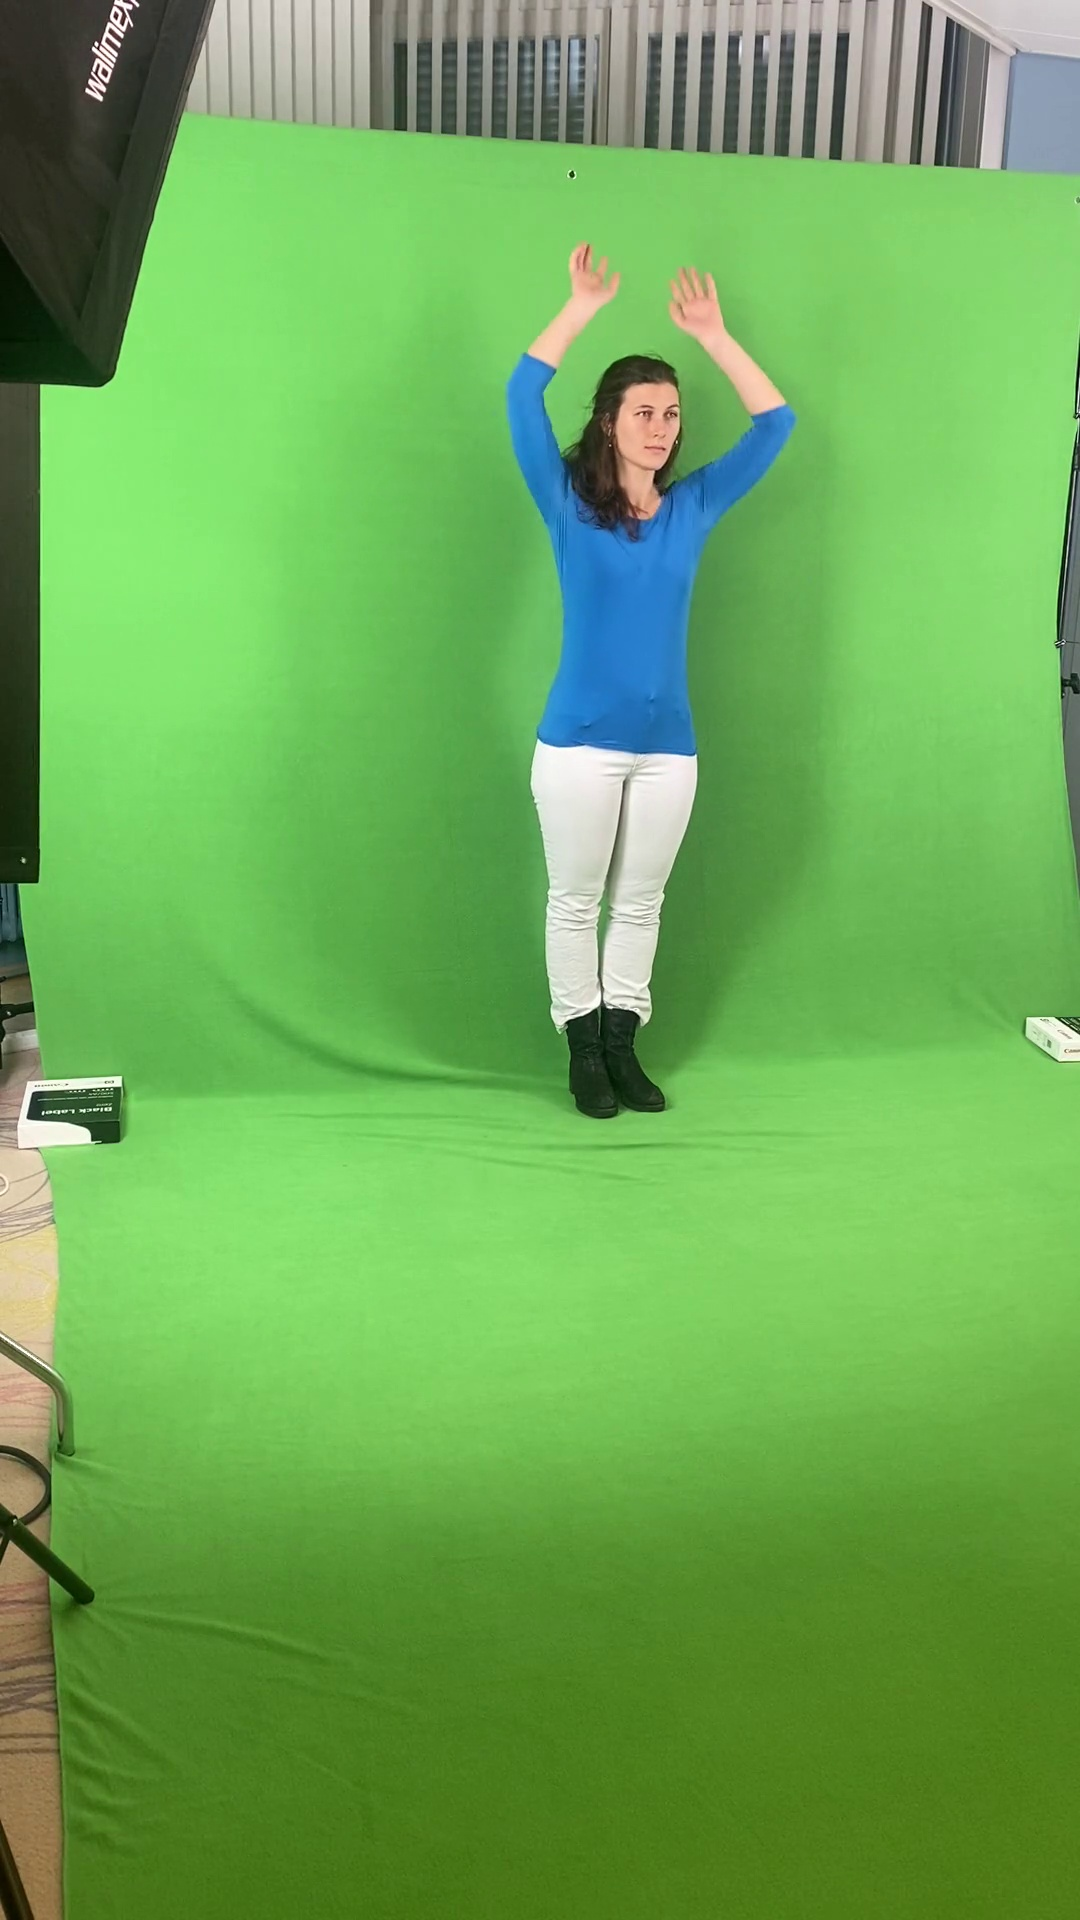
\includegraphics[width=0.187\linewidth]{figures/dataset_images/frame000040.jpg}& 
    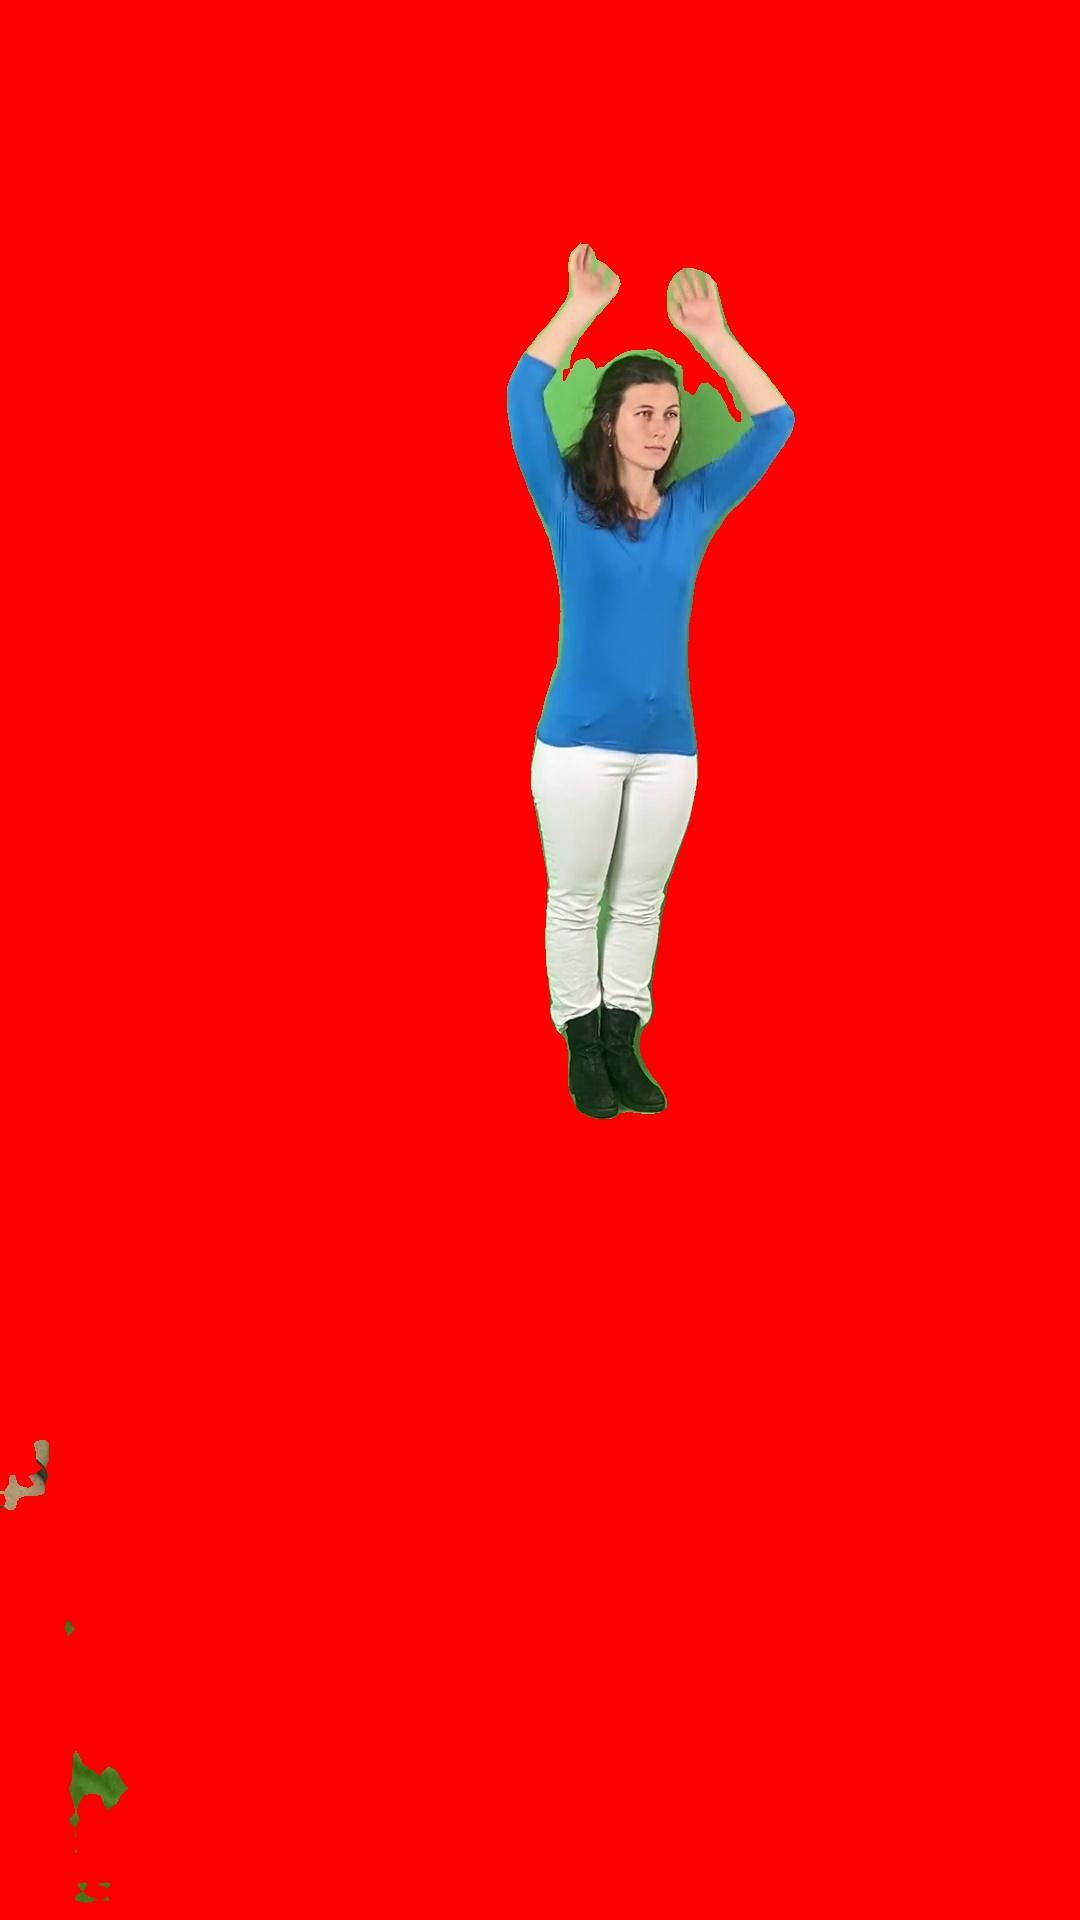
\includegraphics[width=0.187\linewidth]{figures/dataset_images/deeplab_000040.jpg}& 
    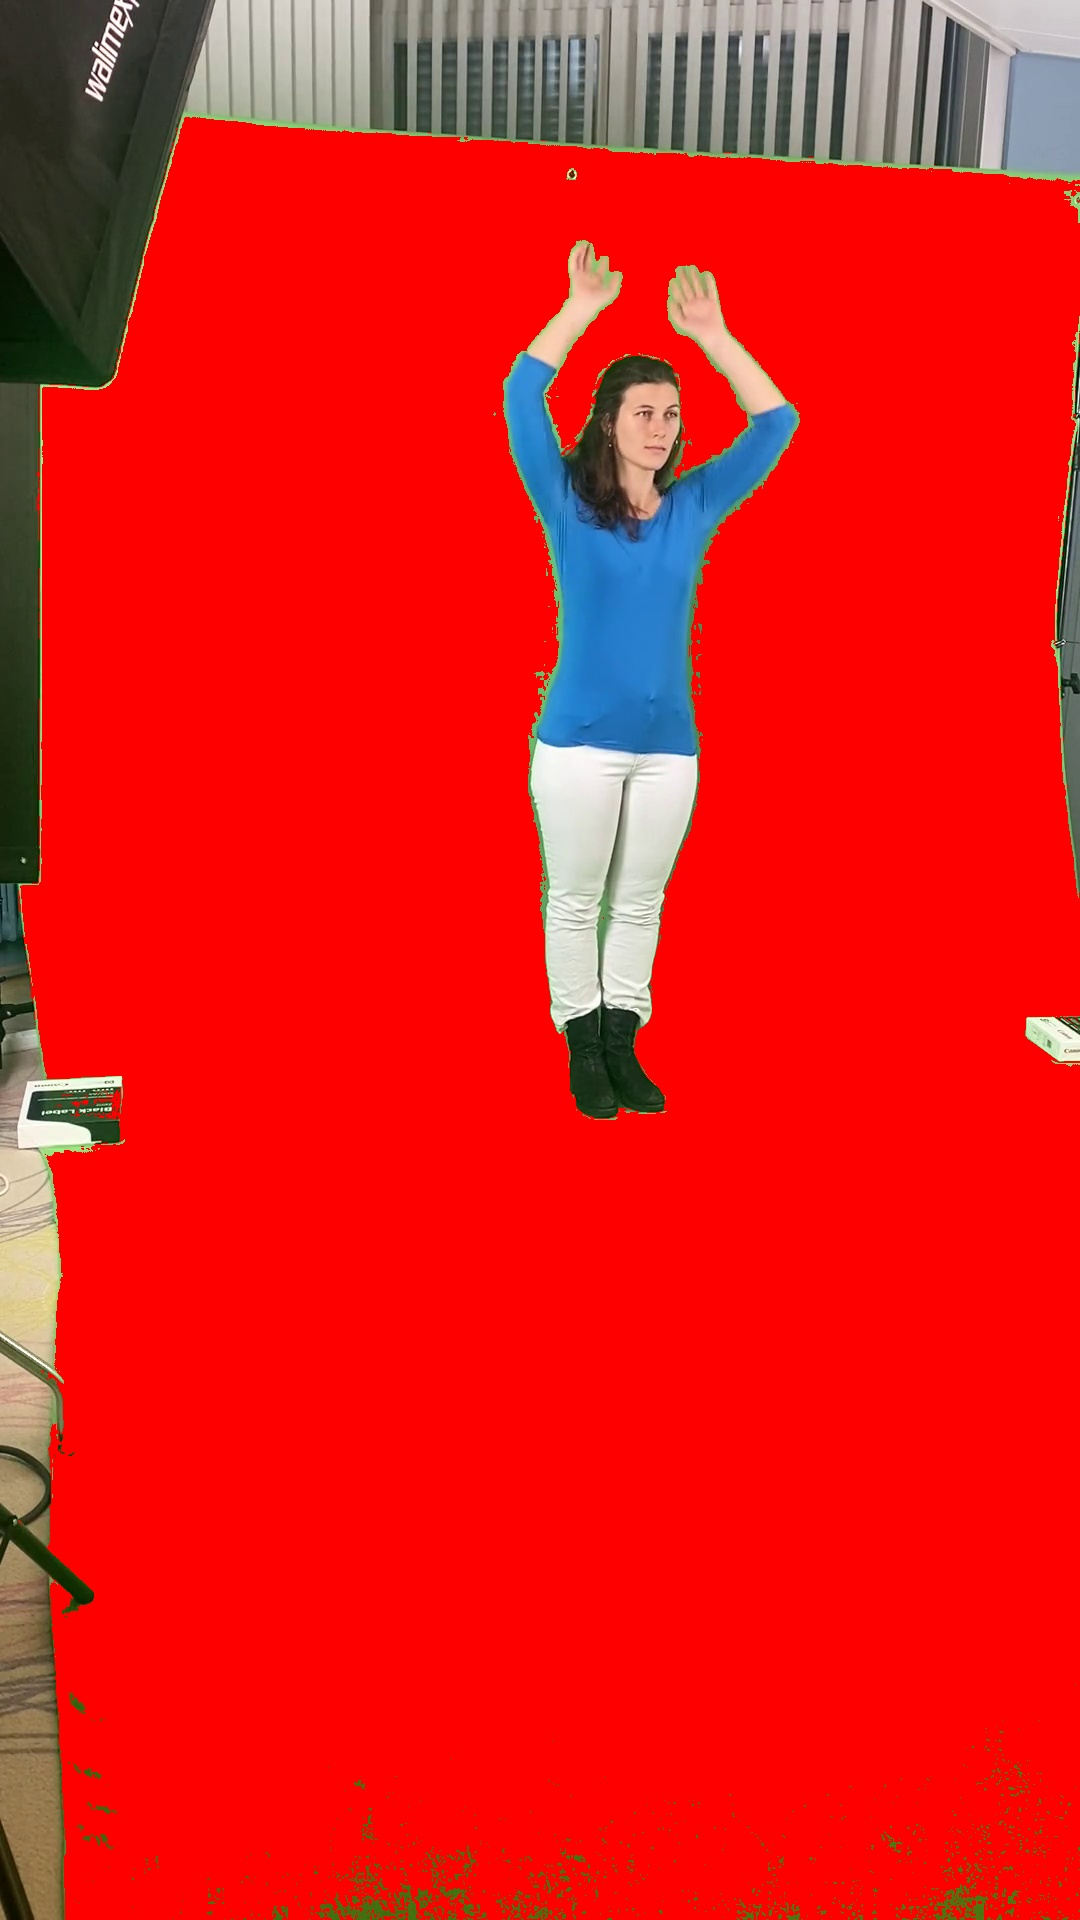
\includegraphics[width=0.187\linewidth]{figures/dataset_images/in_range_000040.jpg}&
    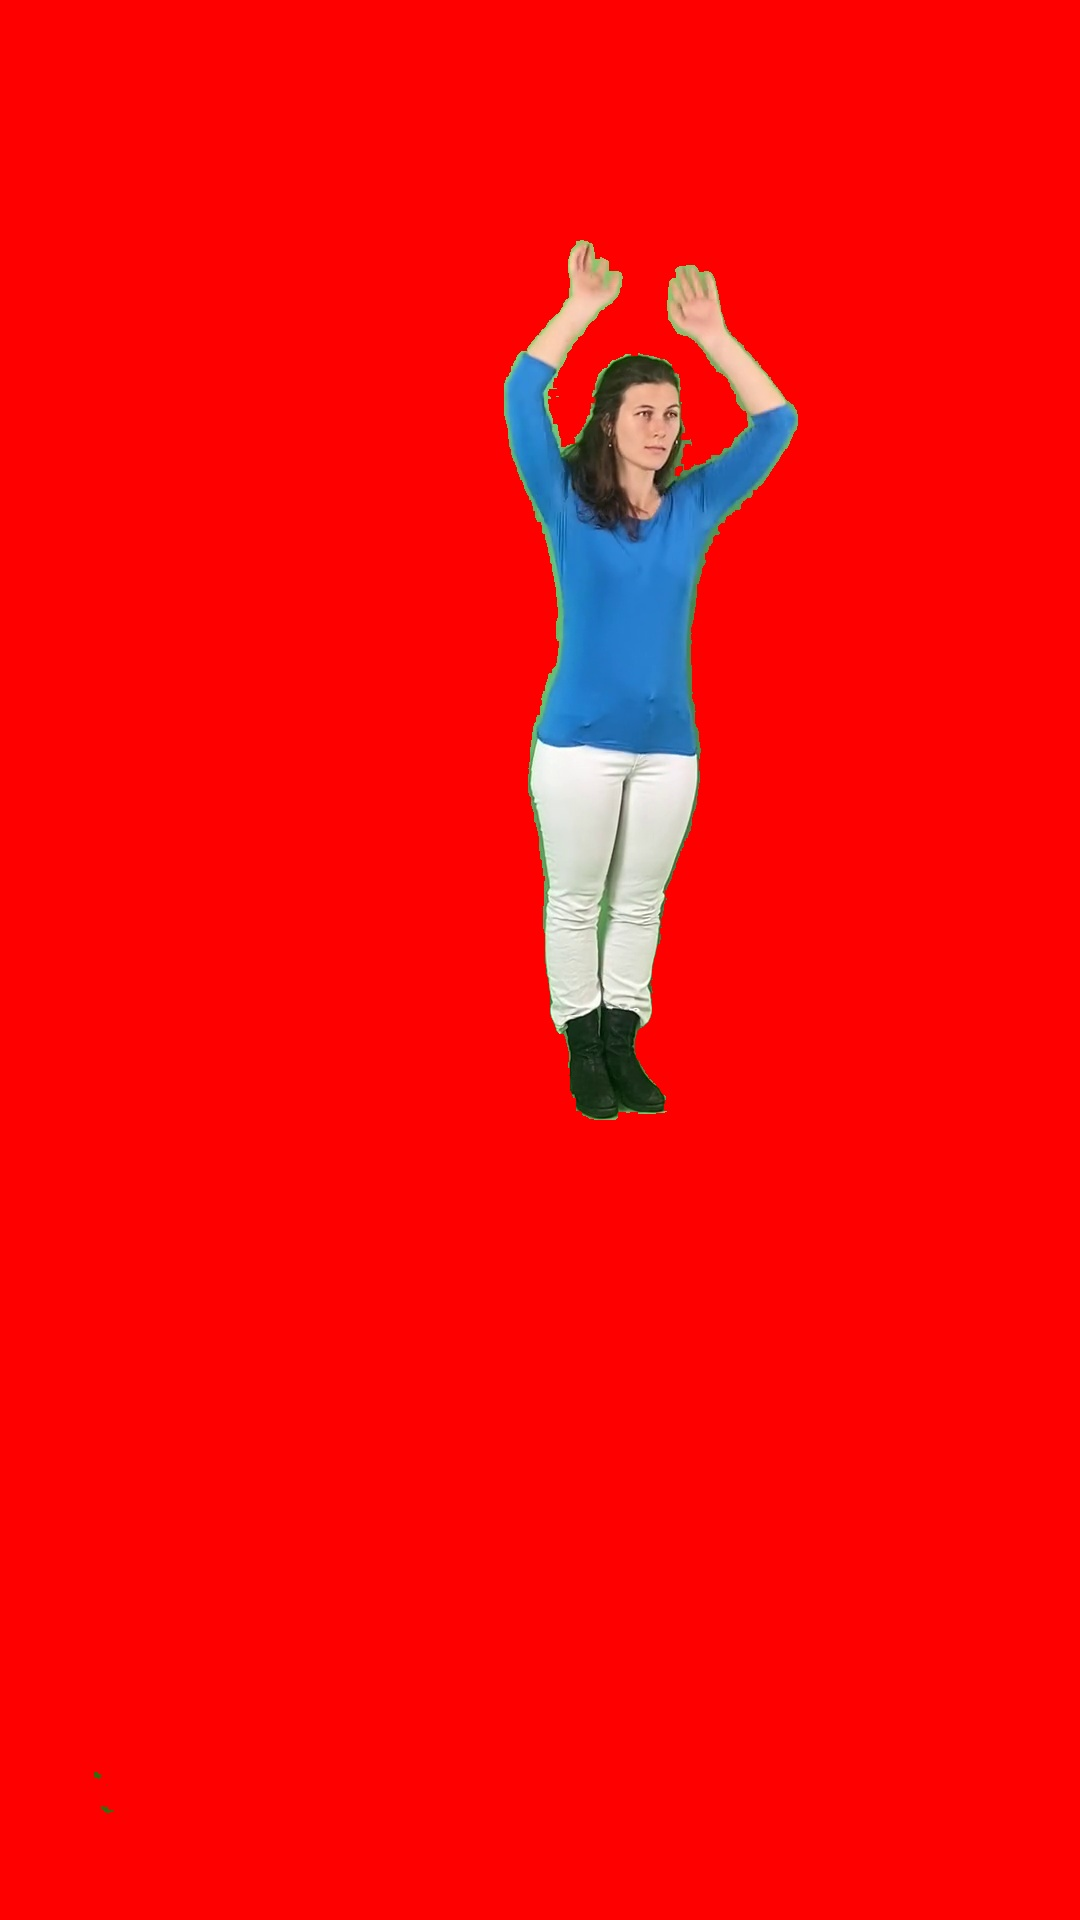
\includegraphics[width=0.187\linewidth]{figures/dataset_images/combined_000040.jpg} \\
    Original frame &(a) & (b) & (c)
  \end{tabular}
  \caption[Generated mask and their binary composition overlayed on the original image]{Generated mask and their binary composition overlayed on the original image
  \textup{(a)} Deeplab output correctly identifies the figure but presents spurious mistake around the arms and at the very bottom. 
  \textup{(b)} Color segmentation presents much sharper boundaries but it's action is limited to the greenscreen. 
  \textup{(c)} Composition of the two binary masks. 
\label{fig: dataset_examples}}
\end{figure}

To fast track the generation of labels we make use of machine predictions instead of  relying on human annotations. 
\begin{figure}
  \centering
  \setlength{\tabcolsep}{0.00530\linewidth}
  % TODO : center the labels
  \begin{tabular}{@{}cccc@{}}
    %  first row
  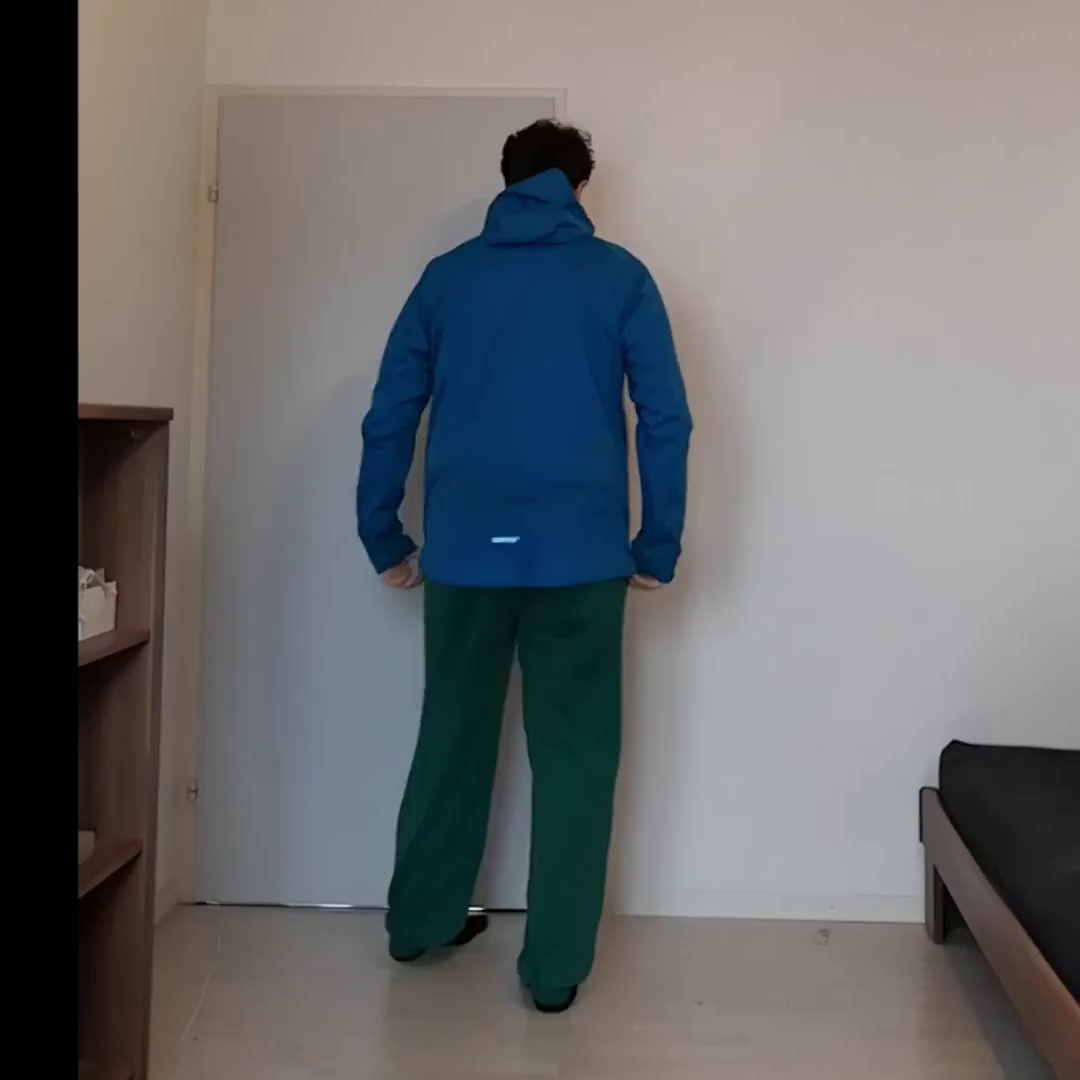
\includegraphics[width=0.187\linewidth]{figures/dataset_images/Dominik_blue_jacket.jpg}&
  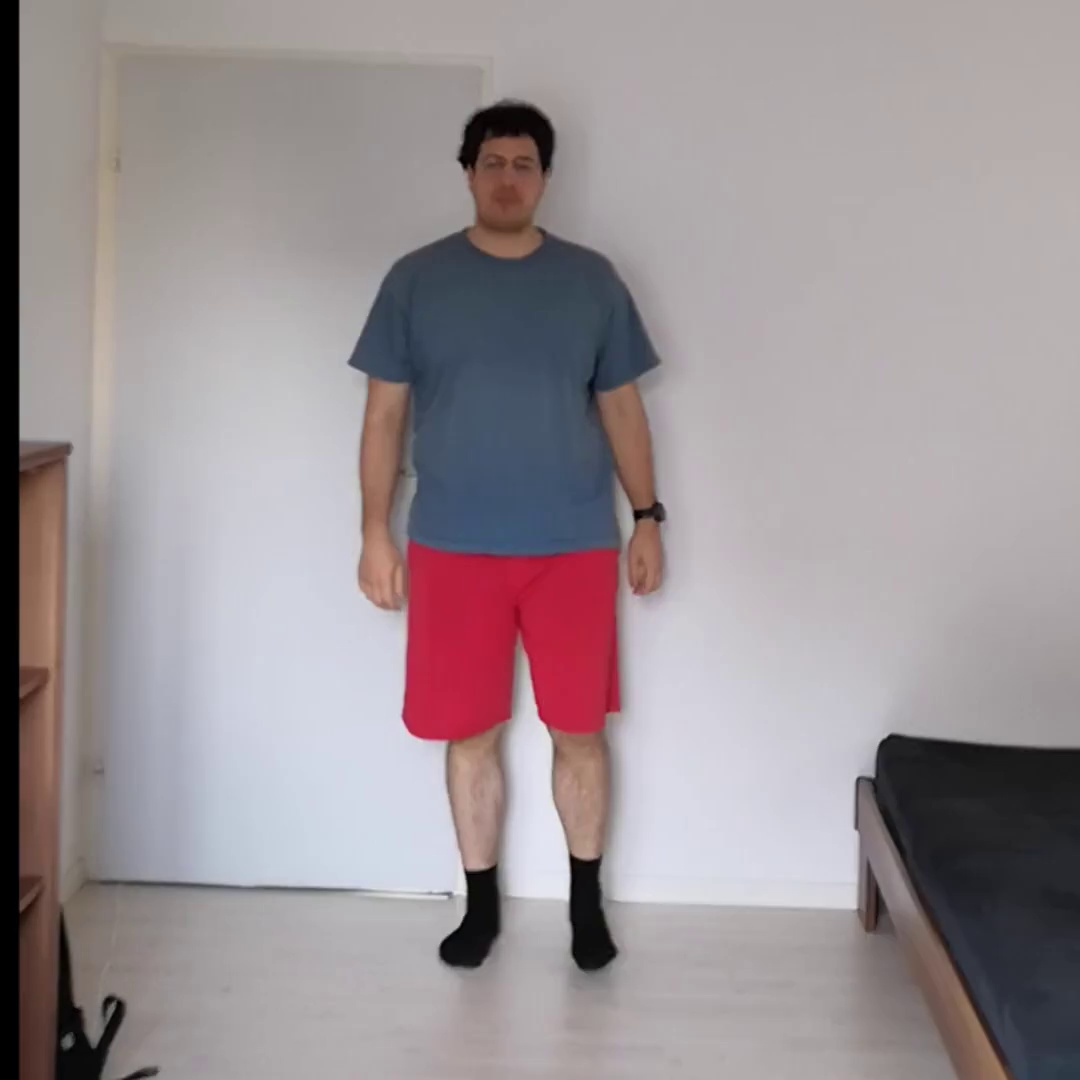
\includegraphics[width=0.187\linewidth]{figures/dataset_images/Dominik_red_pants.jpg}&
  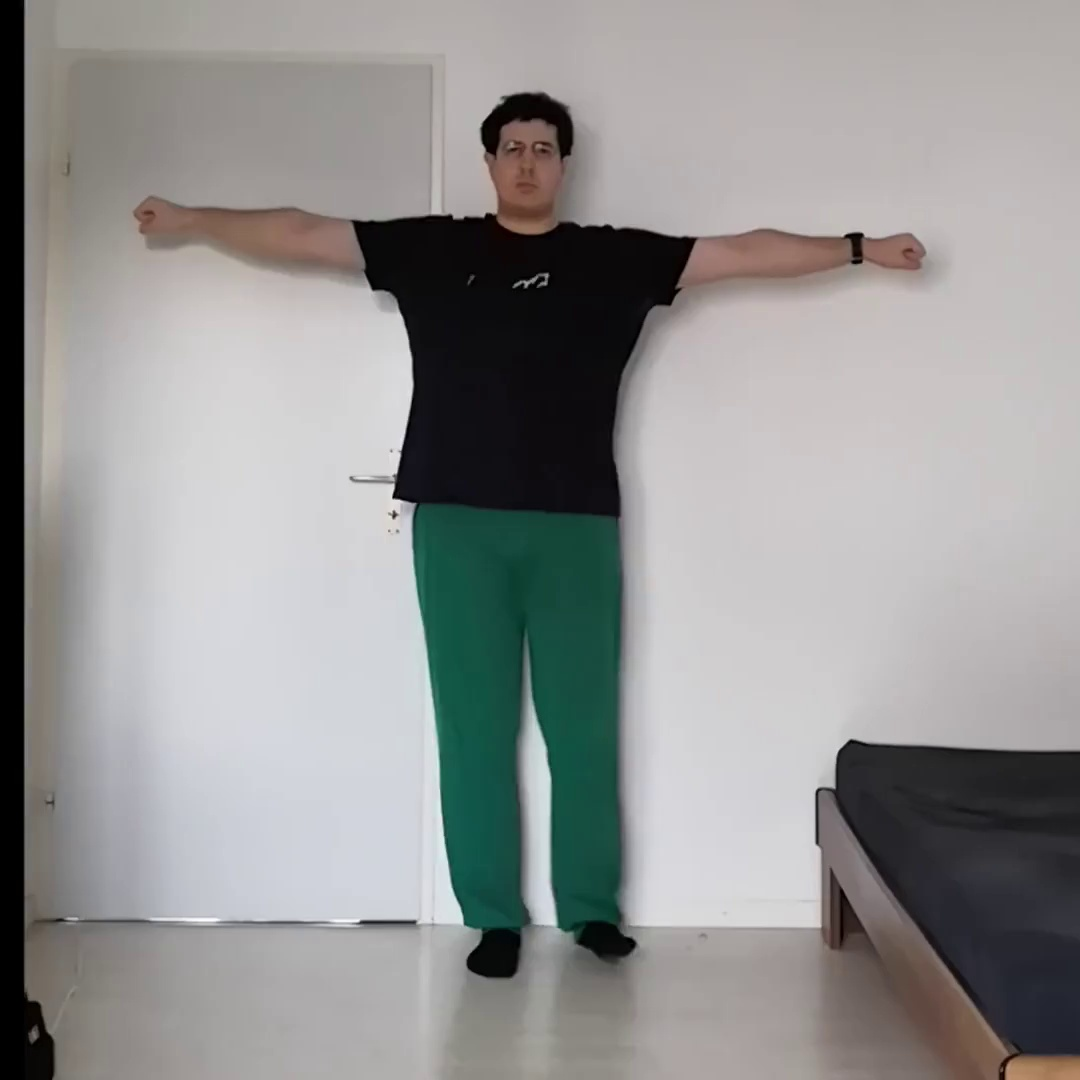
\includegraphics[width=0.187\linewidth]{figures/dataset_images/Dominik_green_pants_black_shirt_01.jpg}&
  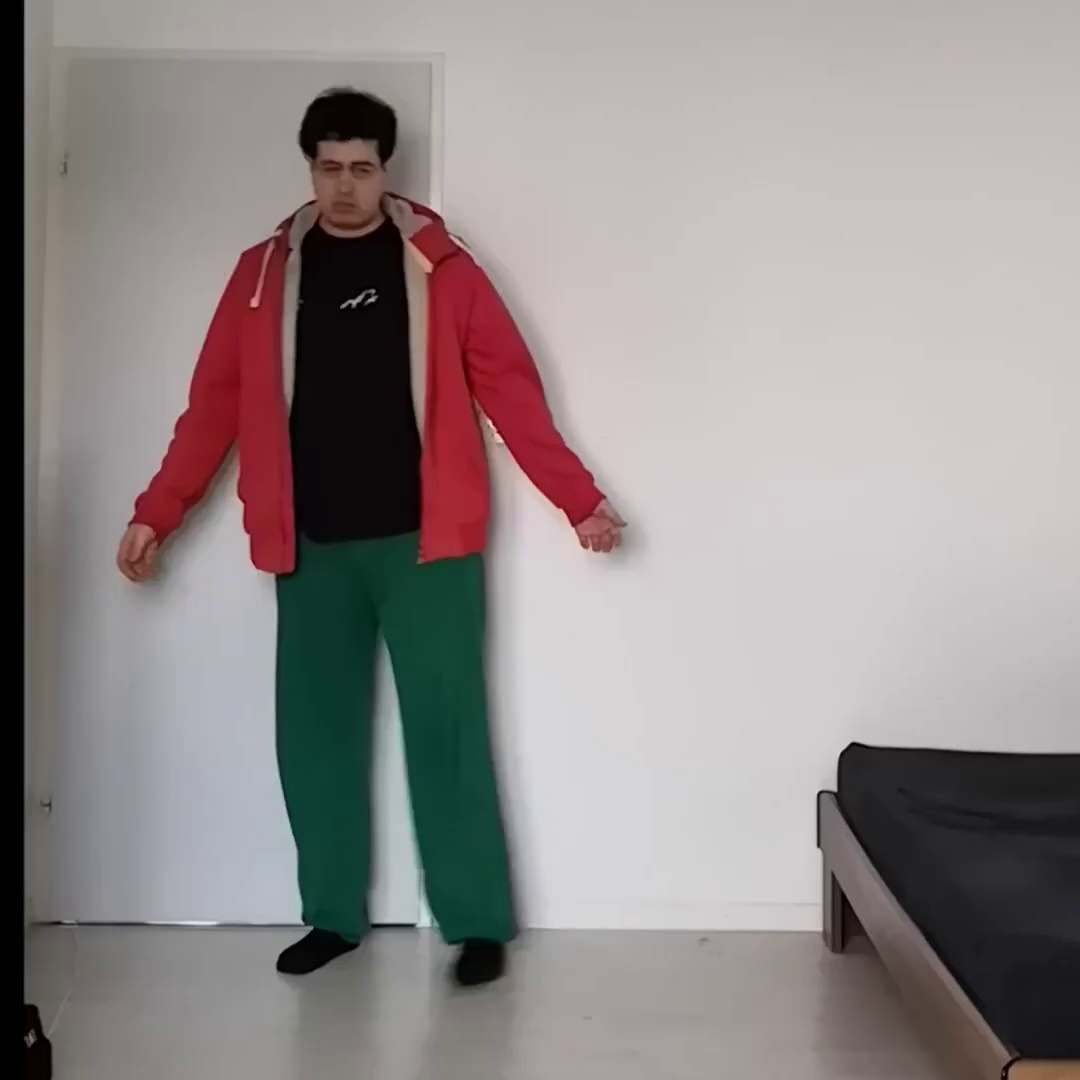
\includegraphics[width=0.187\linewidth]{figures/dataset_images/Dominik_green_pants_red_jacket.jpg}\\
  \centering
  & & (a) \\
    % second row
  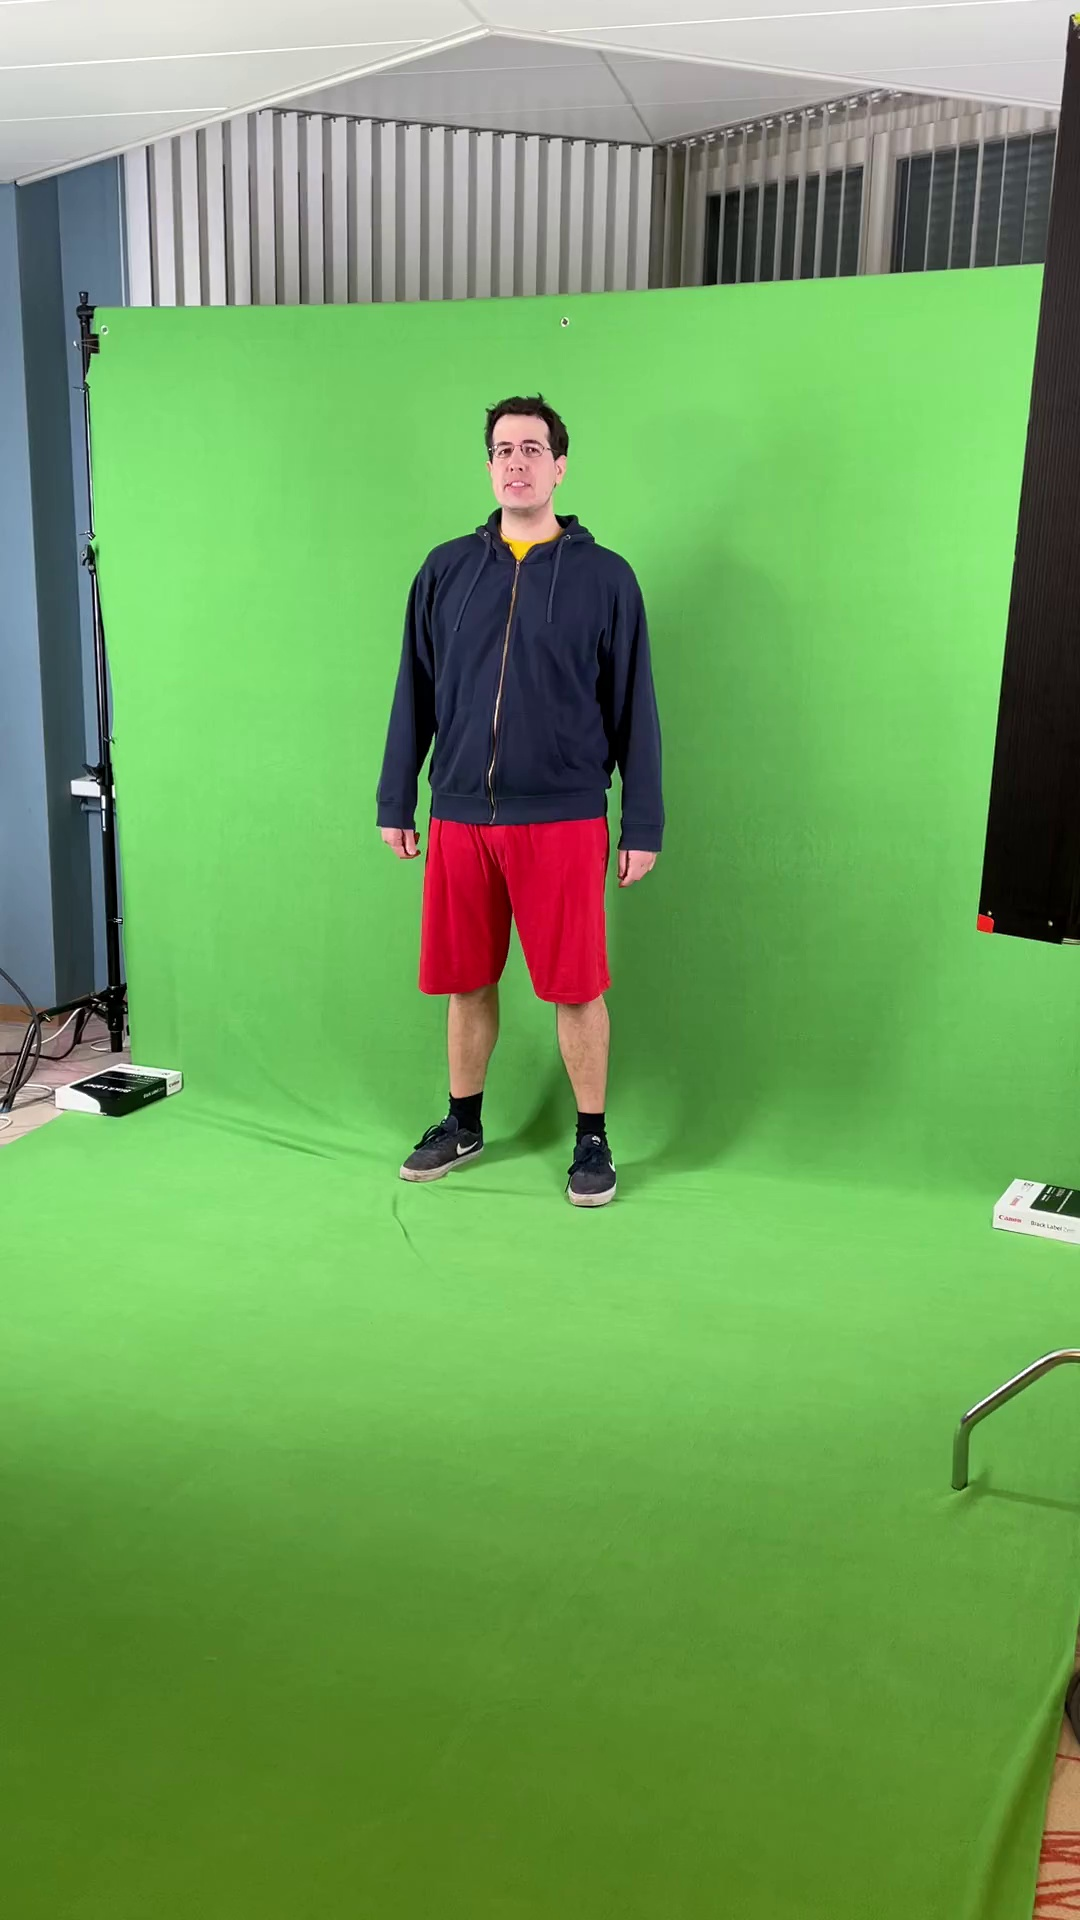
\includegraphics[width=0.187\linewidth]{figures/dataset_images/dominik_green_cloth_shorts_phone1.jpg}&
  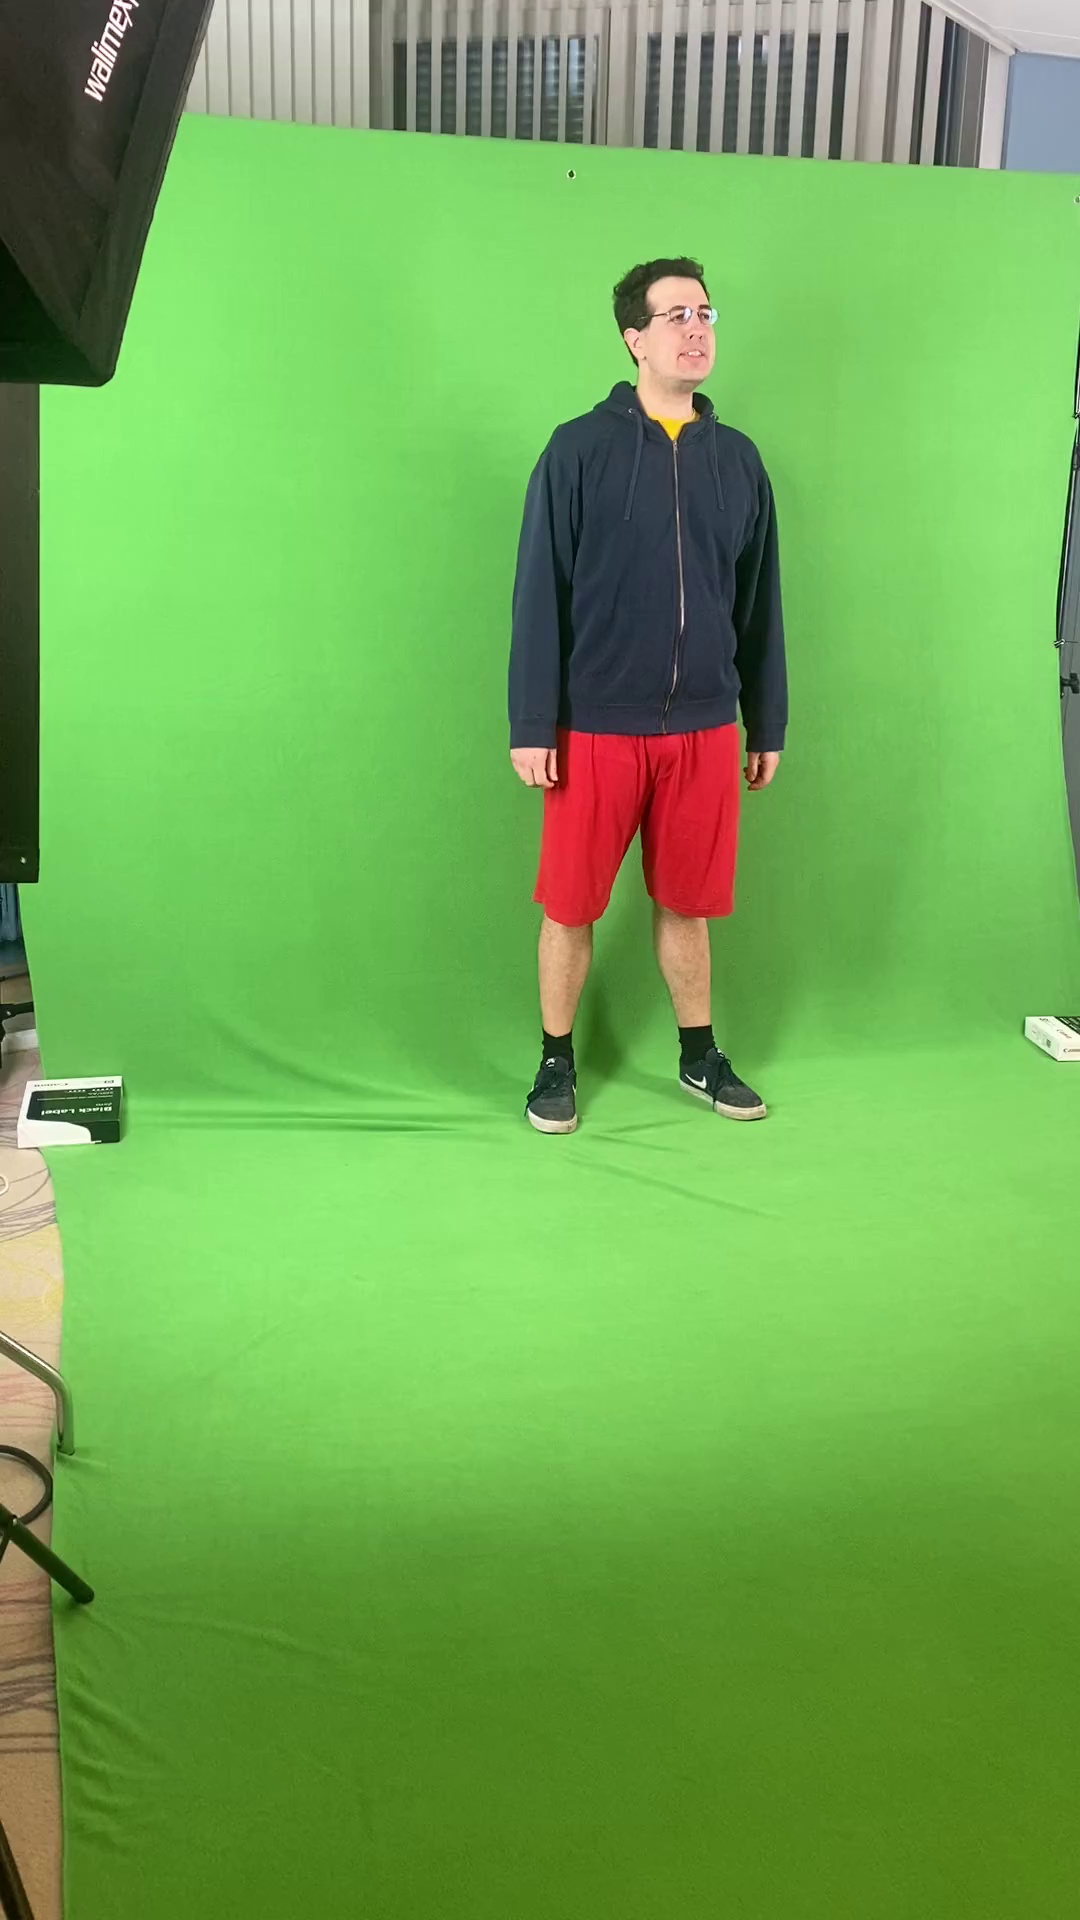
\includegraphics[width=0.187\linewidth]{figures/dataset_images/dominik_green_cloth_shorts_phone2.jpg}&
  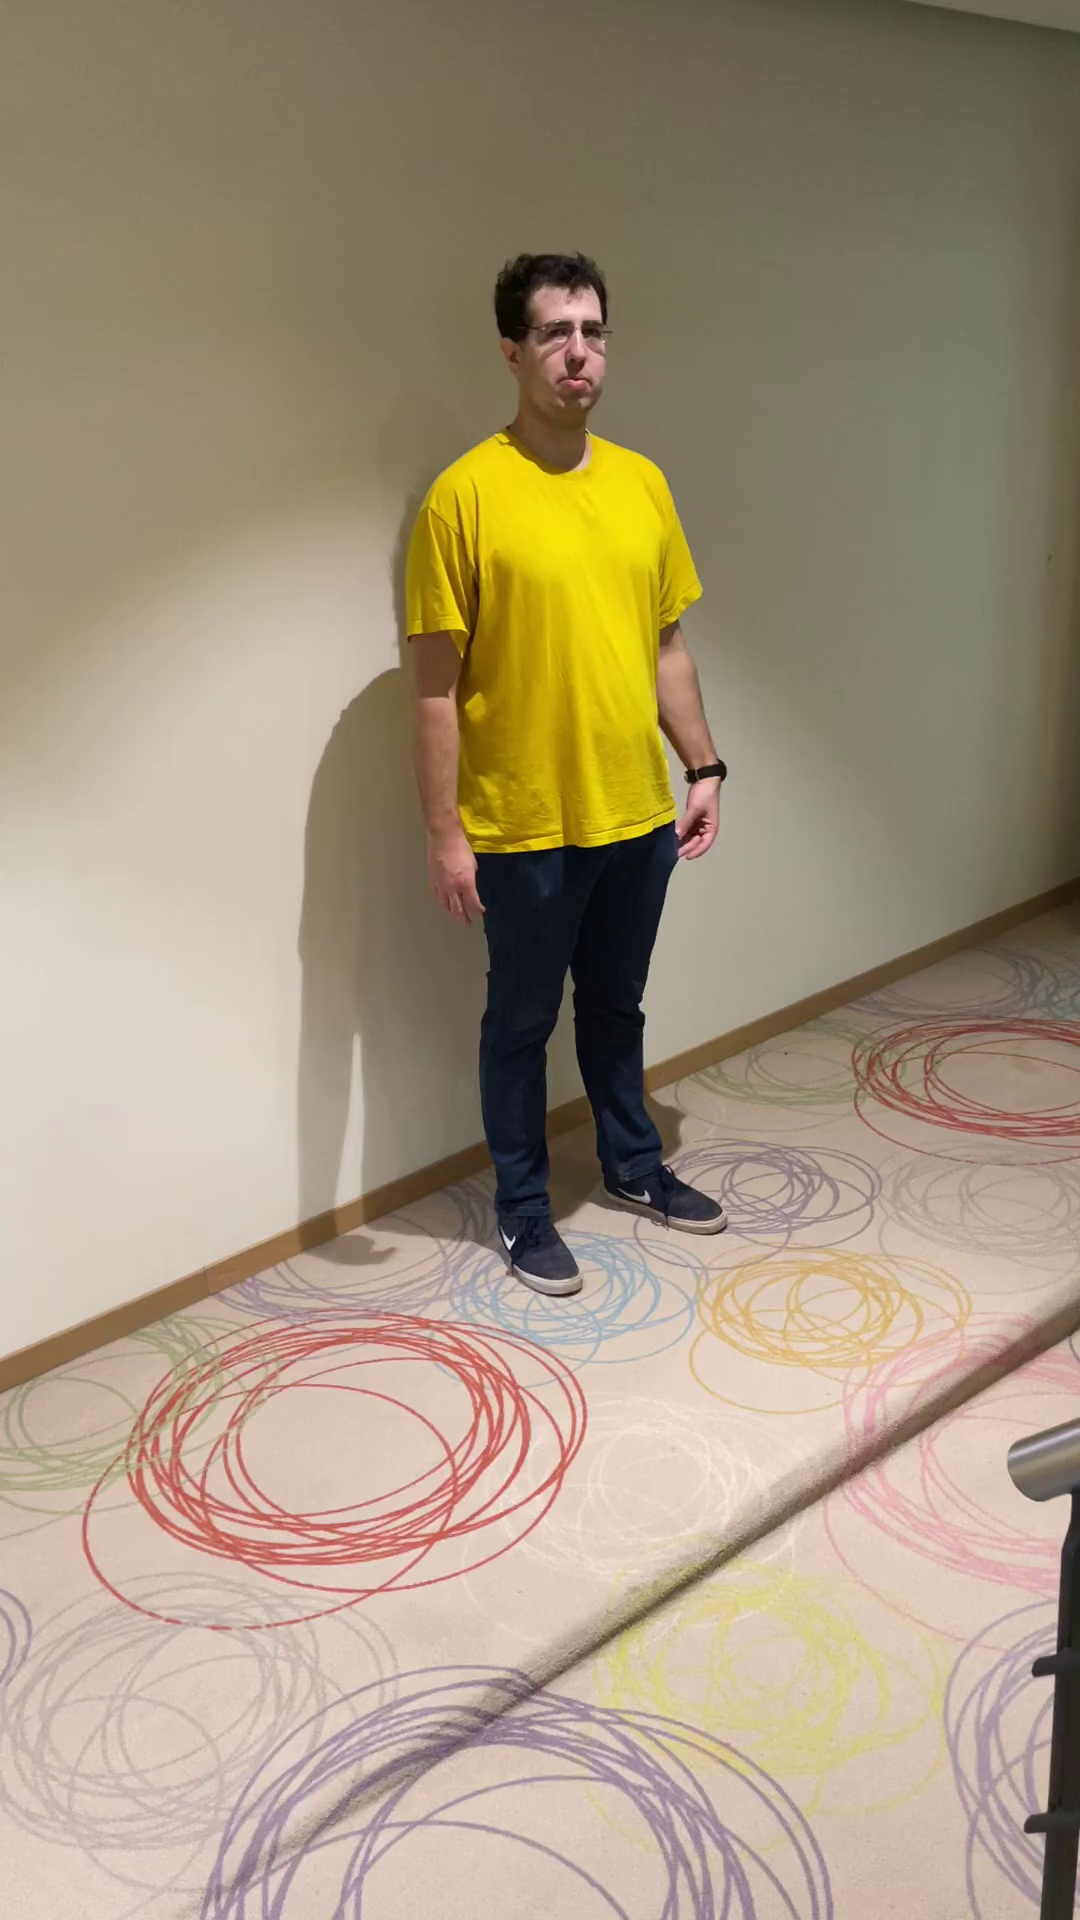
\includegraphics[width=0.187\linewidth]{figures/dataset_images/dominik_stairs_cloth_yellow_phone1.jpg}&
  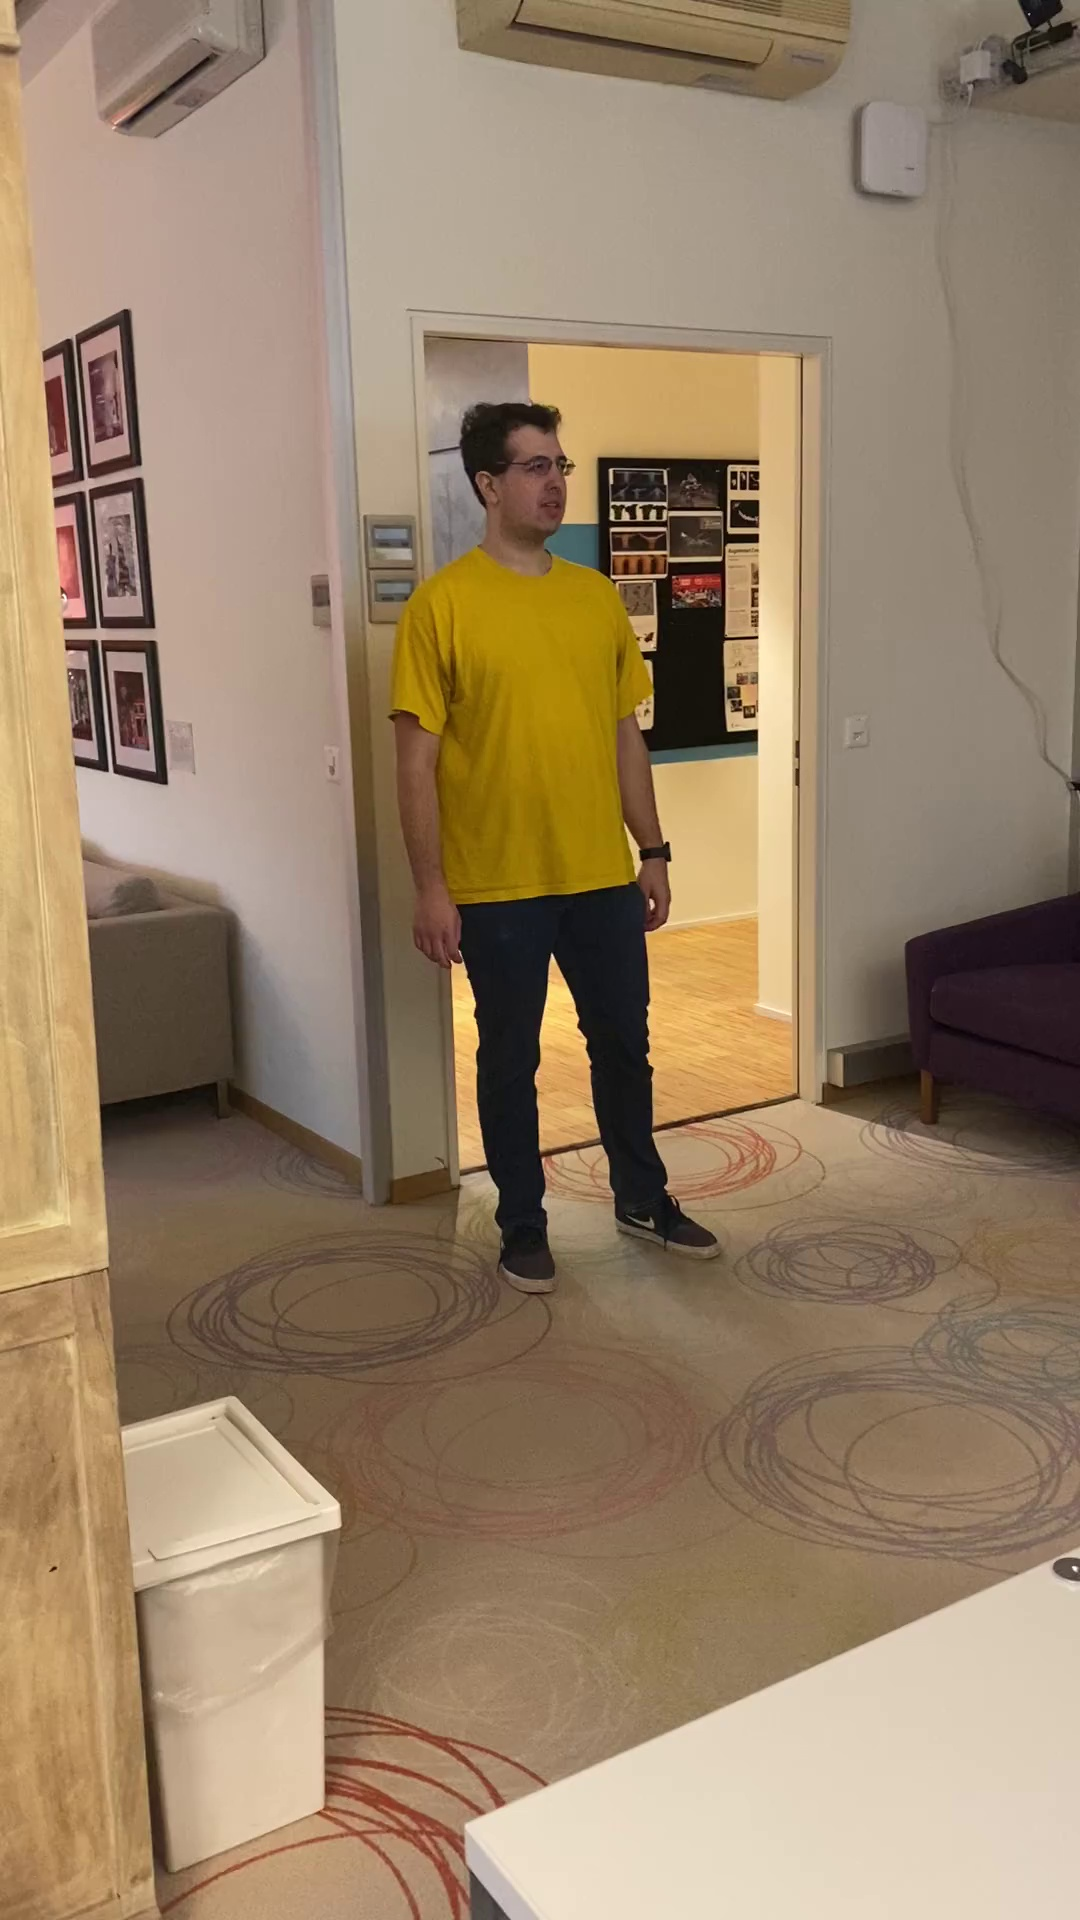
\includegraphics[width=0.187\linewidth]{figures/dataset_images/dominik_office_cloth_yellow_phone2.jpg}\\
  & & (b) \\
    %third row
  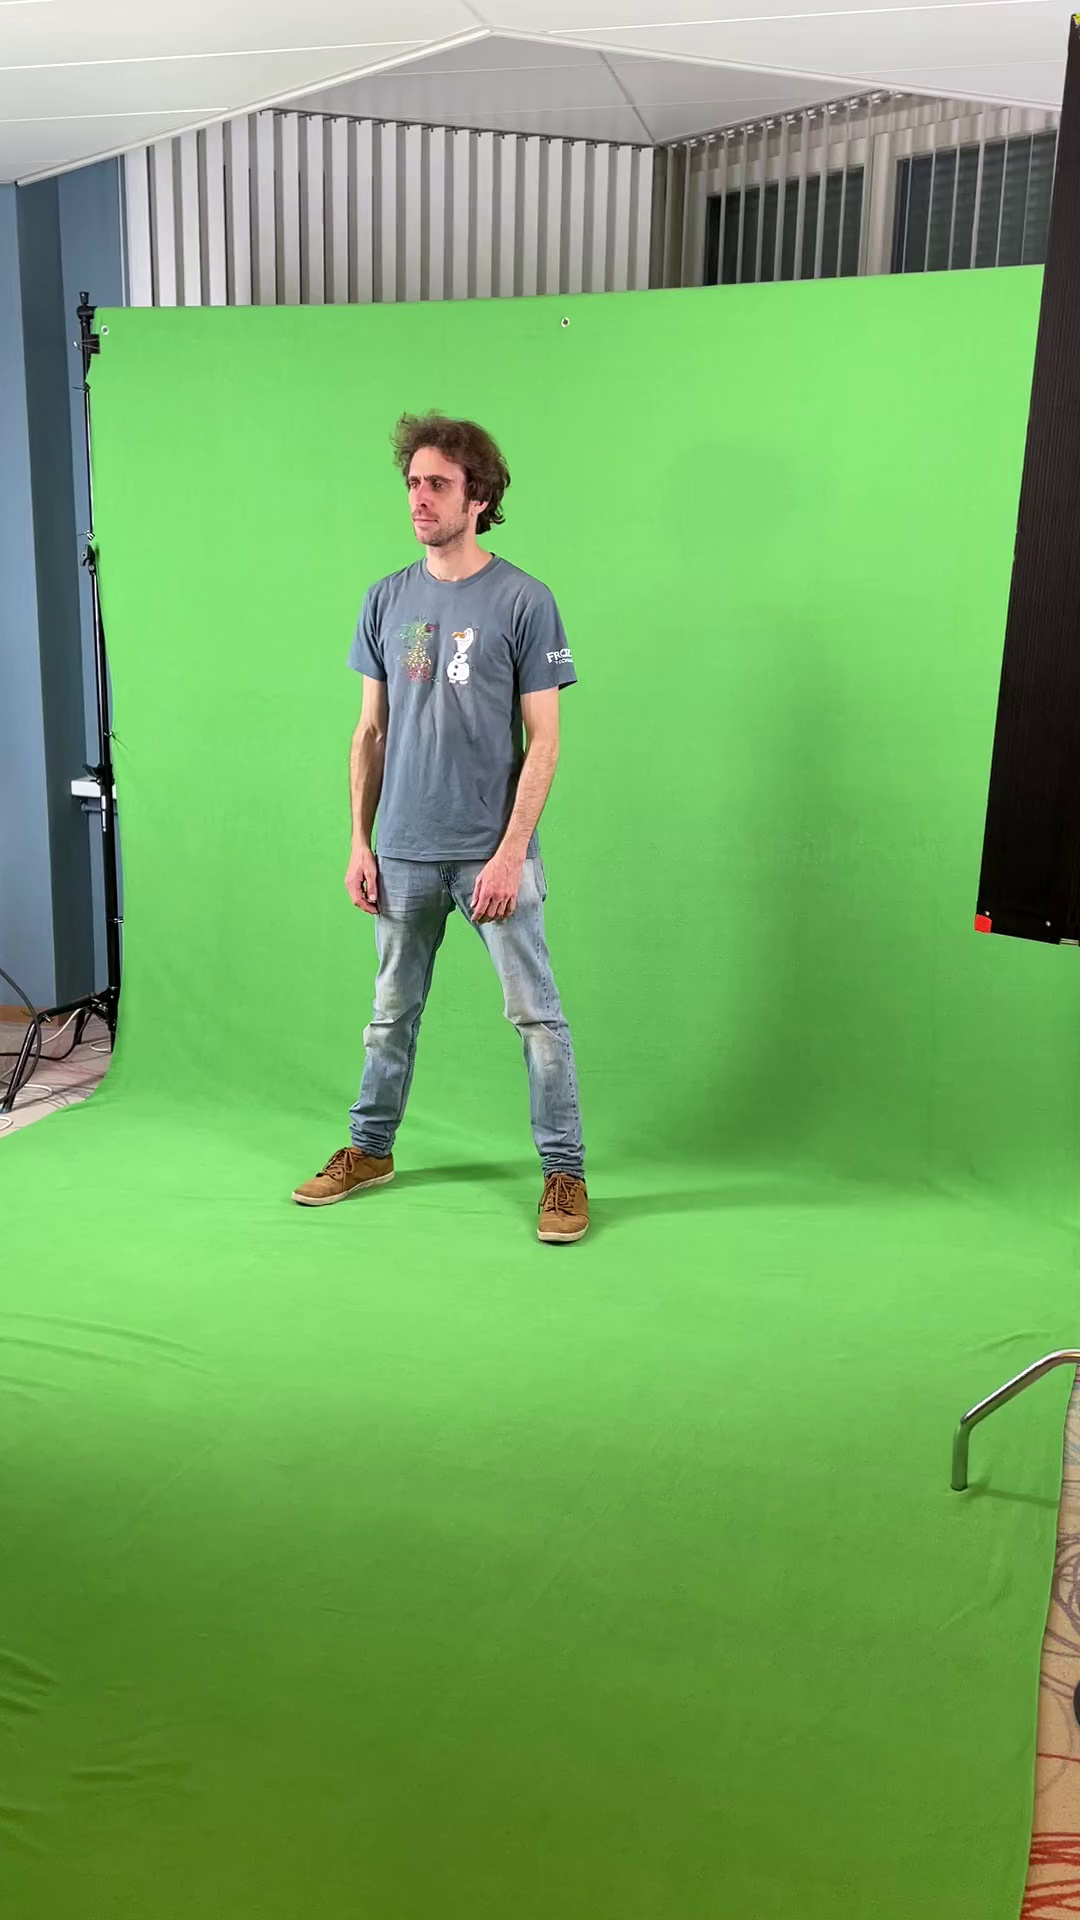
\includegraphics[width=0.187\linewidth]{figures/dataset_images/mattia_green_cloth_short_phone1.jpg}&
  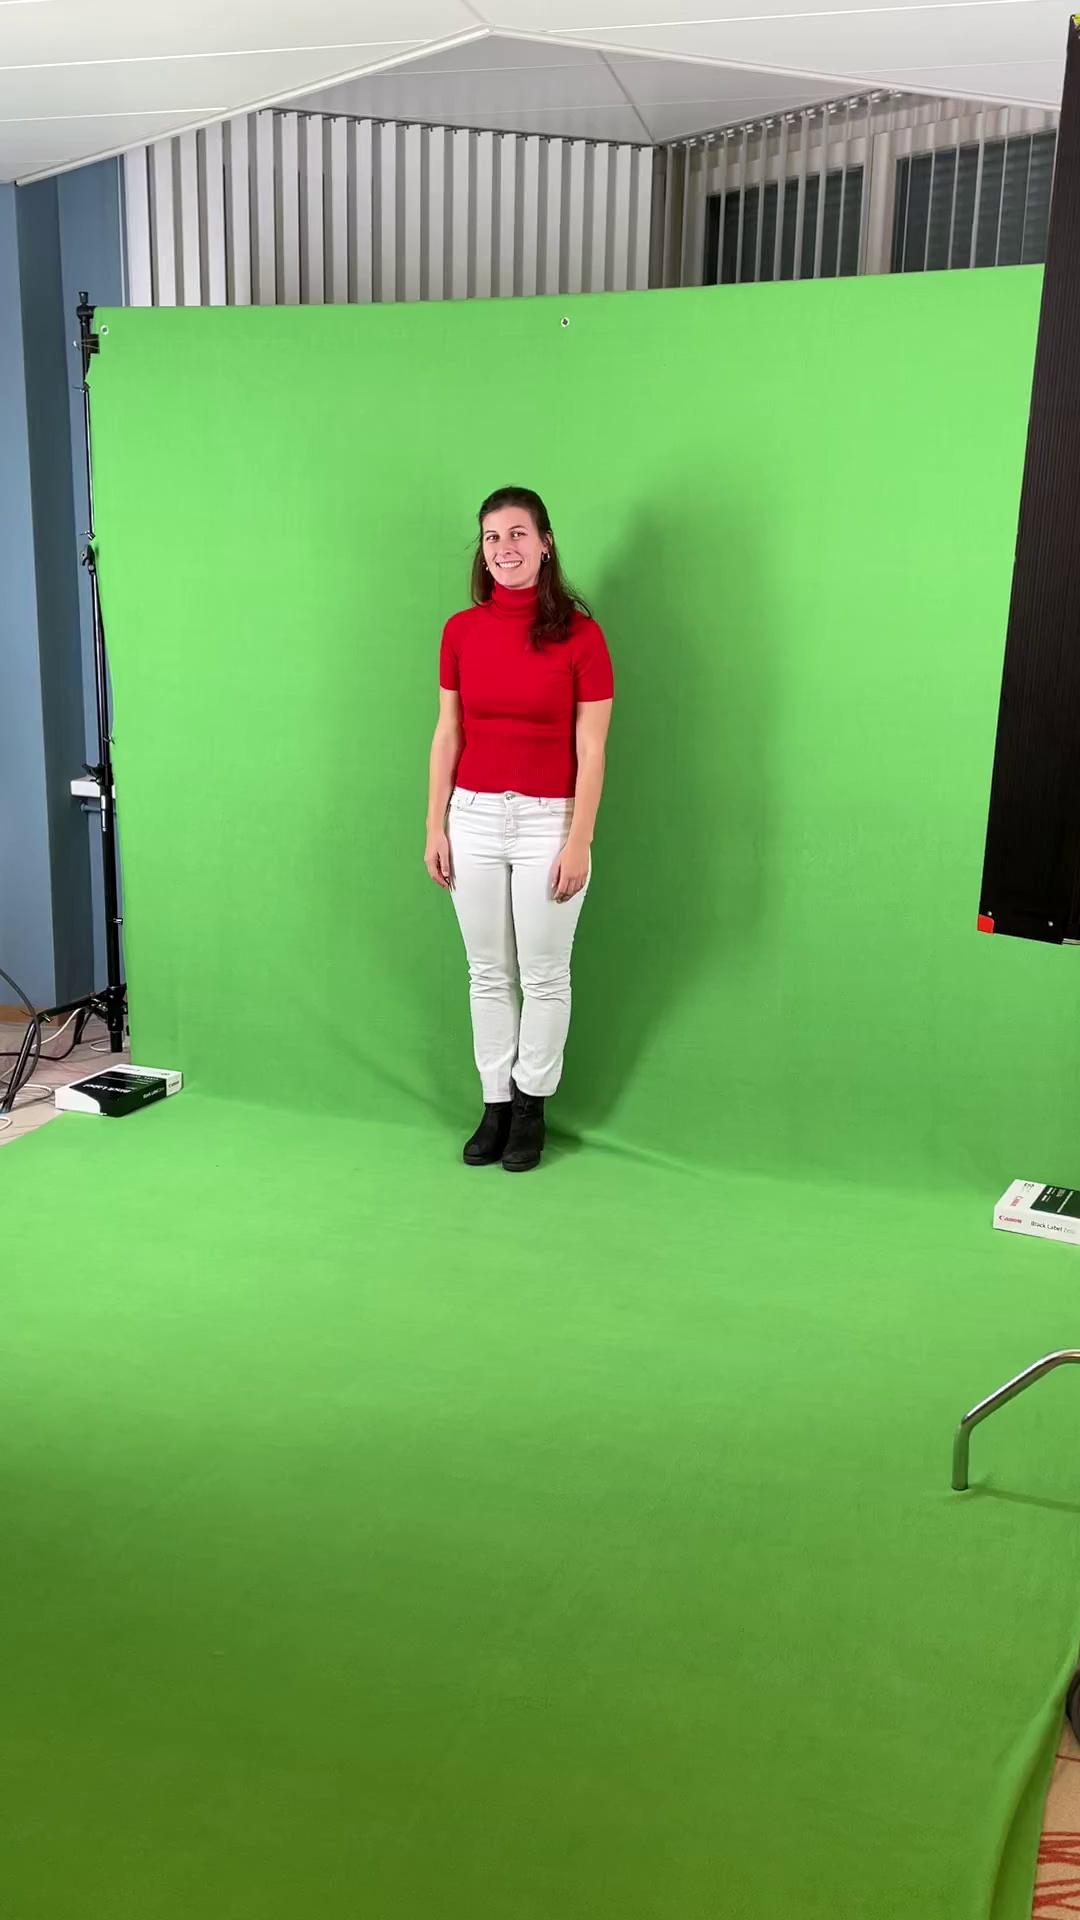
\includegraphics[width=0.187\linewidth]{figures/dataset_images/francesca_green_cloth_red_phone1.jpg}&
  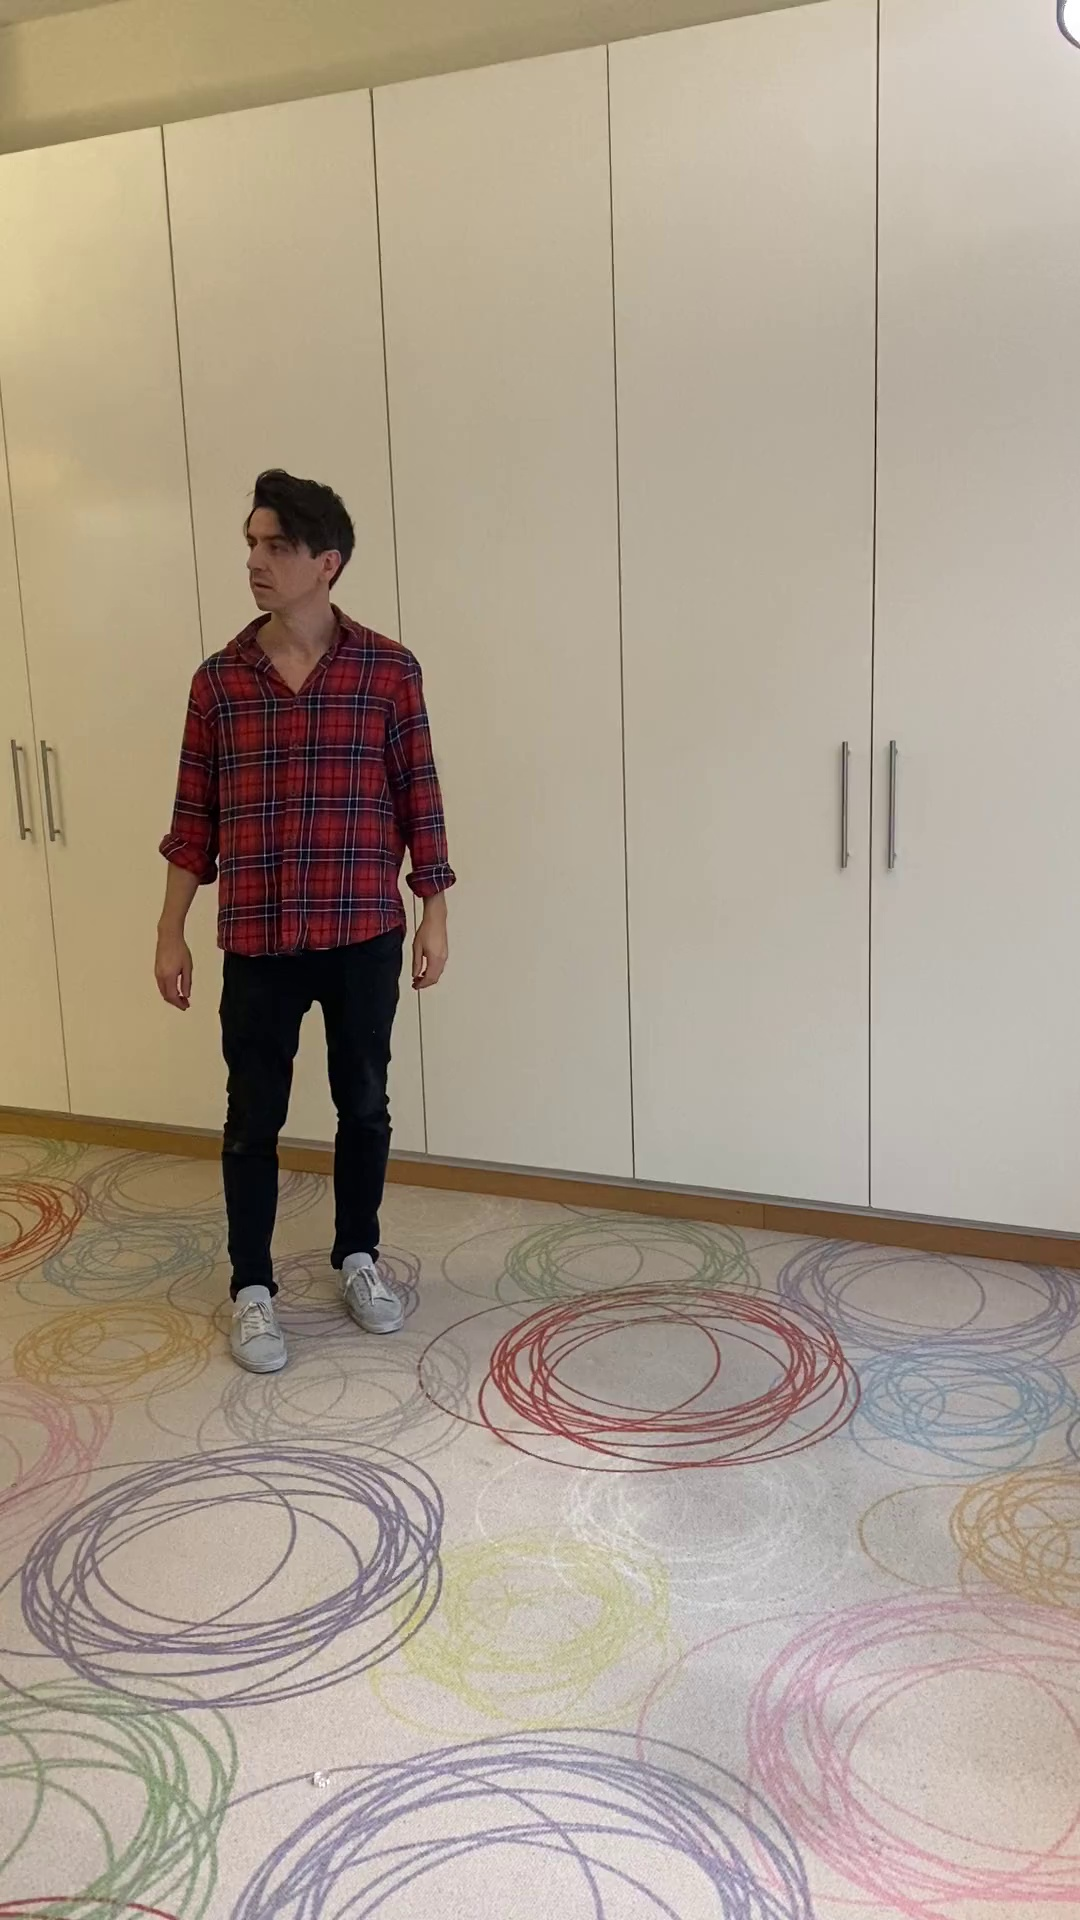
\includegraphics[width=0.187\linewidth]{figures/dataset_images/martin_cubard_cloth_red_phone2.jpg}&
  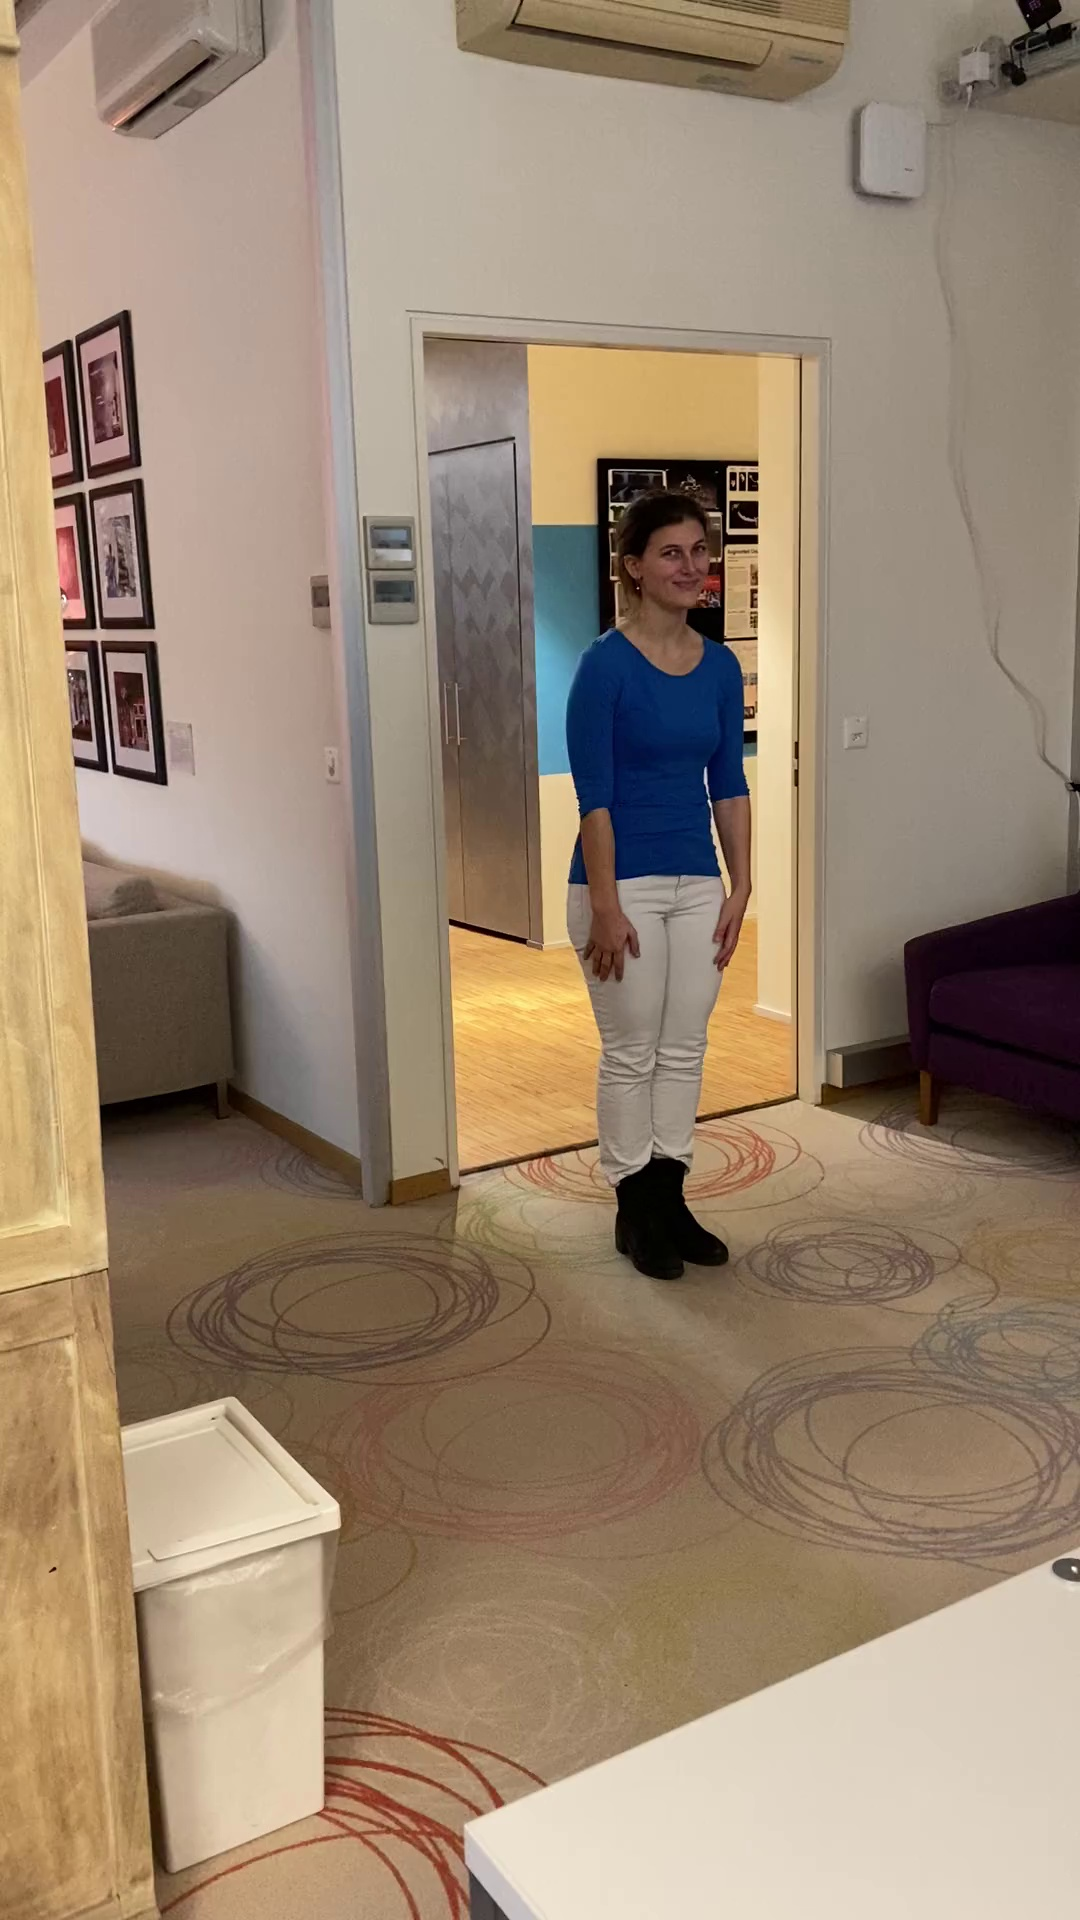
\includegraphics[width=0.187\linewidth]{figures/dataset_images/francesca_office_cloth_blue_phone2.jpg}\\
  & &(c)
  \end{tabular}
  \caption[Samples from the created dataset]{Samples from the created dataset.
      \textup{(a)} Four different appearance in the single camera view.
      \textup{(b)} One take from each camera from the dual camera setup with greenscreen as background, two takes with a background "in the wild"
      \textup{(c)} Other subjects.
    \label{fig: dataset_examples}}
\end{figure}


These come in two variants: 
\begin{itemize}
  \item labels are generated with baseline OpenPose network. This relies on a single camera view setting 
  % \item introduce the issue of visibility? 
  % \item explain in Related work how the 3D skeleton is generated
  \item labels are obtained throughun the projection of the 3D skeleton back into the camera view.
\end{itemize}



Such examples may act as noise
and pollute the learned model if the model is not
rich enough to capture such appearance variability.


One
could start by arguing that the reason is not that datasets are
bad, but that our object representations and recognition algorithms are terrible and end up over-learning aspects of the
visual data that relates to the dataset and not to the ultimate
visual task
\section{Training on 2D data}
\label{section: training on 2D data}

\section{Triangulated experiments}
label{section: training on 3D data}


\subsection{Validation method}

\begin{figure}
  \centering
  \begin{tabular}{@{}cc@{}}
    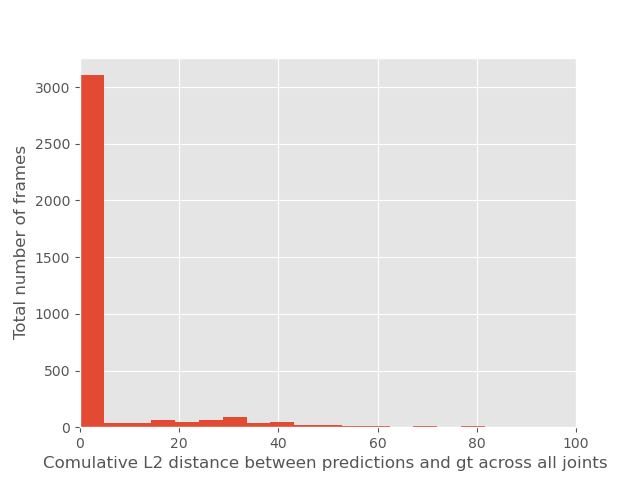
\includegraphics[height=0.487\linewidth]{figures/hist_diff_to_handlabel.png}&
    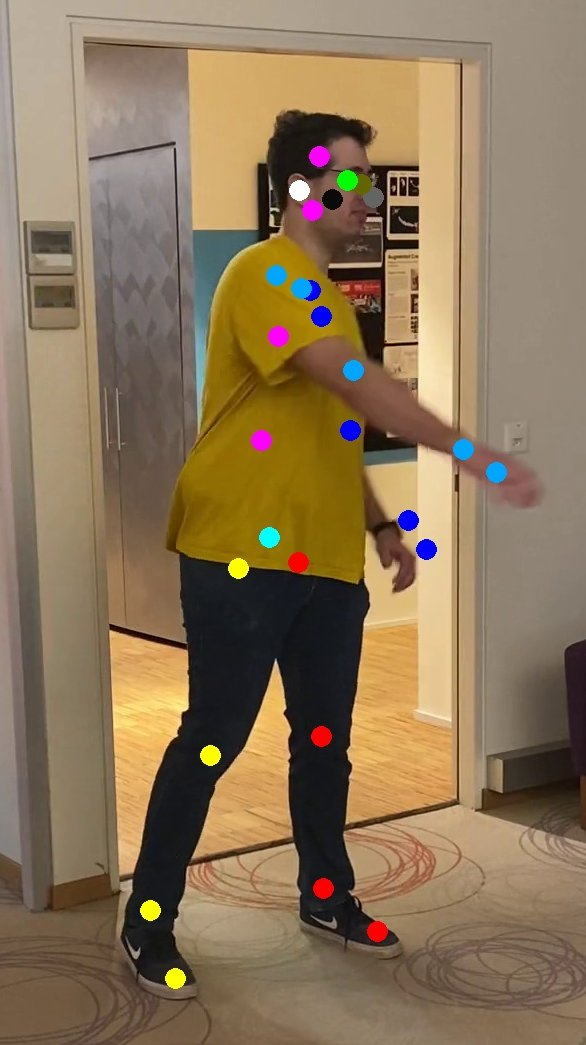
\includegraphics[height=0.487\linewidth]{figures/dominik_office_cloth_yellow_phone2_40.jpg}\\
    (a)&(b)\\
    \end{tabular}
  \caption{ 
    \textup{(a)}   Distribution of the errors between the triangulated projected point and ground truth. Only the comulative errors across all joints is considered here. Deviations of around 20 pixels from ground truth, (example in figure  \textup{(b)}) can be considered relevant : during the generation of ground truth labels small deviations as the well most face keypoints were left unchanged. Around 550 frames, out of the 3685 needed adjustment..
    \label{fig:comulative_3D_predictions_errors}
     }
\end{figure}
It seems improbable that  

\subsection{}

\begin{table}
    \centering
    \begin{tabular}{|l|p{0.4\linewidth}|}
    \hline
    \emph{Quant.} & \emph{Ingredient}\\
    \hline
		200g &Wei{\ss}mehl\\
		1/4  &Packung Frischhefe\\
		4EL  &lauwarme Milch\\
		4EL  &Öl\\
		1TL  &Zucker\\
		1TL  &Salz\\
		&lauwarmes Wasser\\
    \hline
    \end{tabular}
    \caption[Flammkuchenteig]{Flammkuchenteig. The ingredients have to be carefully chosen.\label{tab:mytable}}
\end{table}
%
Lorem ipsum dolor sit amet, consectetuer adipiscing elit, sed diam nonummy nibh euismod tincidunt ut laoreet dolore magna aliquam erat volutpat. Ut wisi enim ad minim veniam, quis nostrud exerci tation ullamcorper suscipit lobortis nisl ut aliquip ex ea commodo consequat, see Table~\ref{tab:mytable}. Duis autem vel eum iriure dolor in hendrerit in vulputate velit esse molestie consequat, vel illum dolore eu feugiat nulla facilisis at vero et accumsan et iusto odio dignissim qui blandit praesent luptatum zzril delenit augue duis dolore te feugait nulla facilisi. Lorem ipsum dolor sit amet, consectetuer adipiscing elit, sed diam,
see Figure~\ref{fig:voldiff}~(a).
%
\begin{figure}
    \centering
    \setlength{\tabcolsep}{0.0130\linewidth}
    \begin{tabular}{@{}cc@{}}
    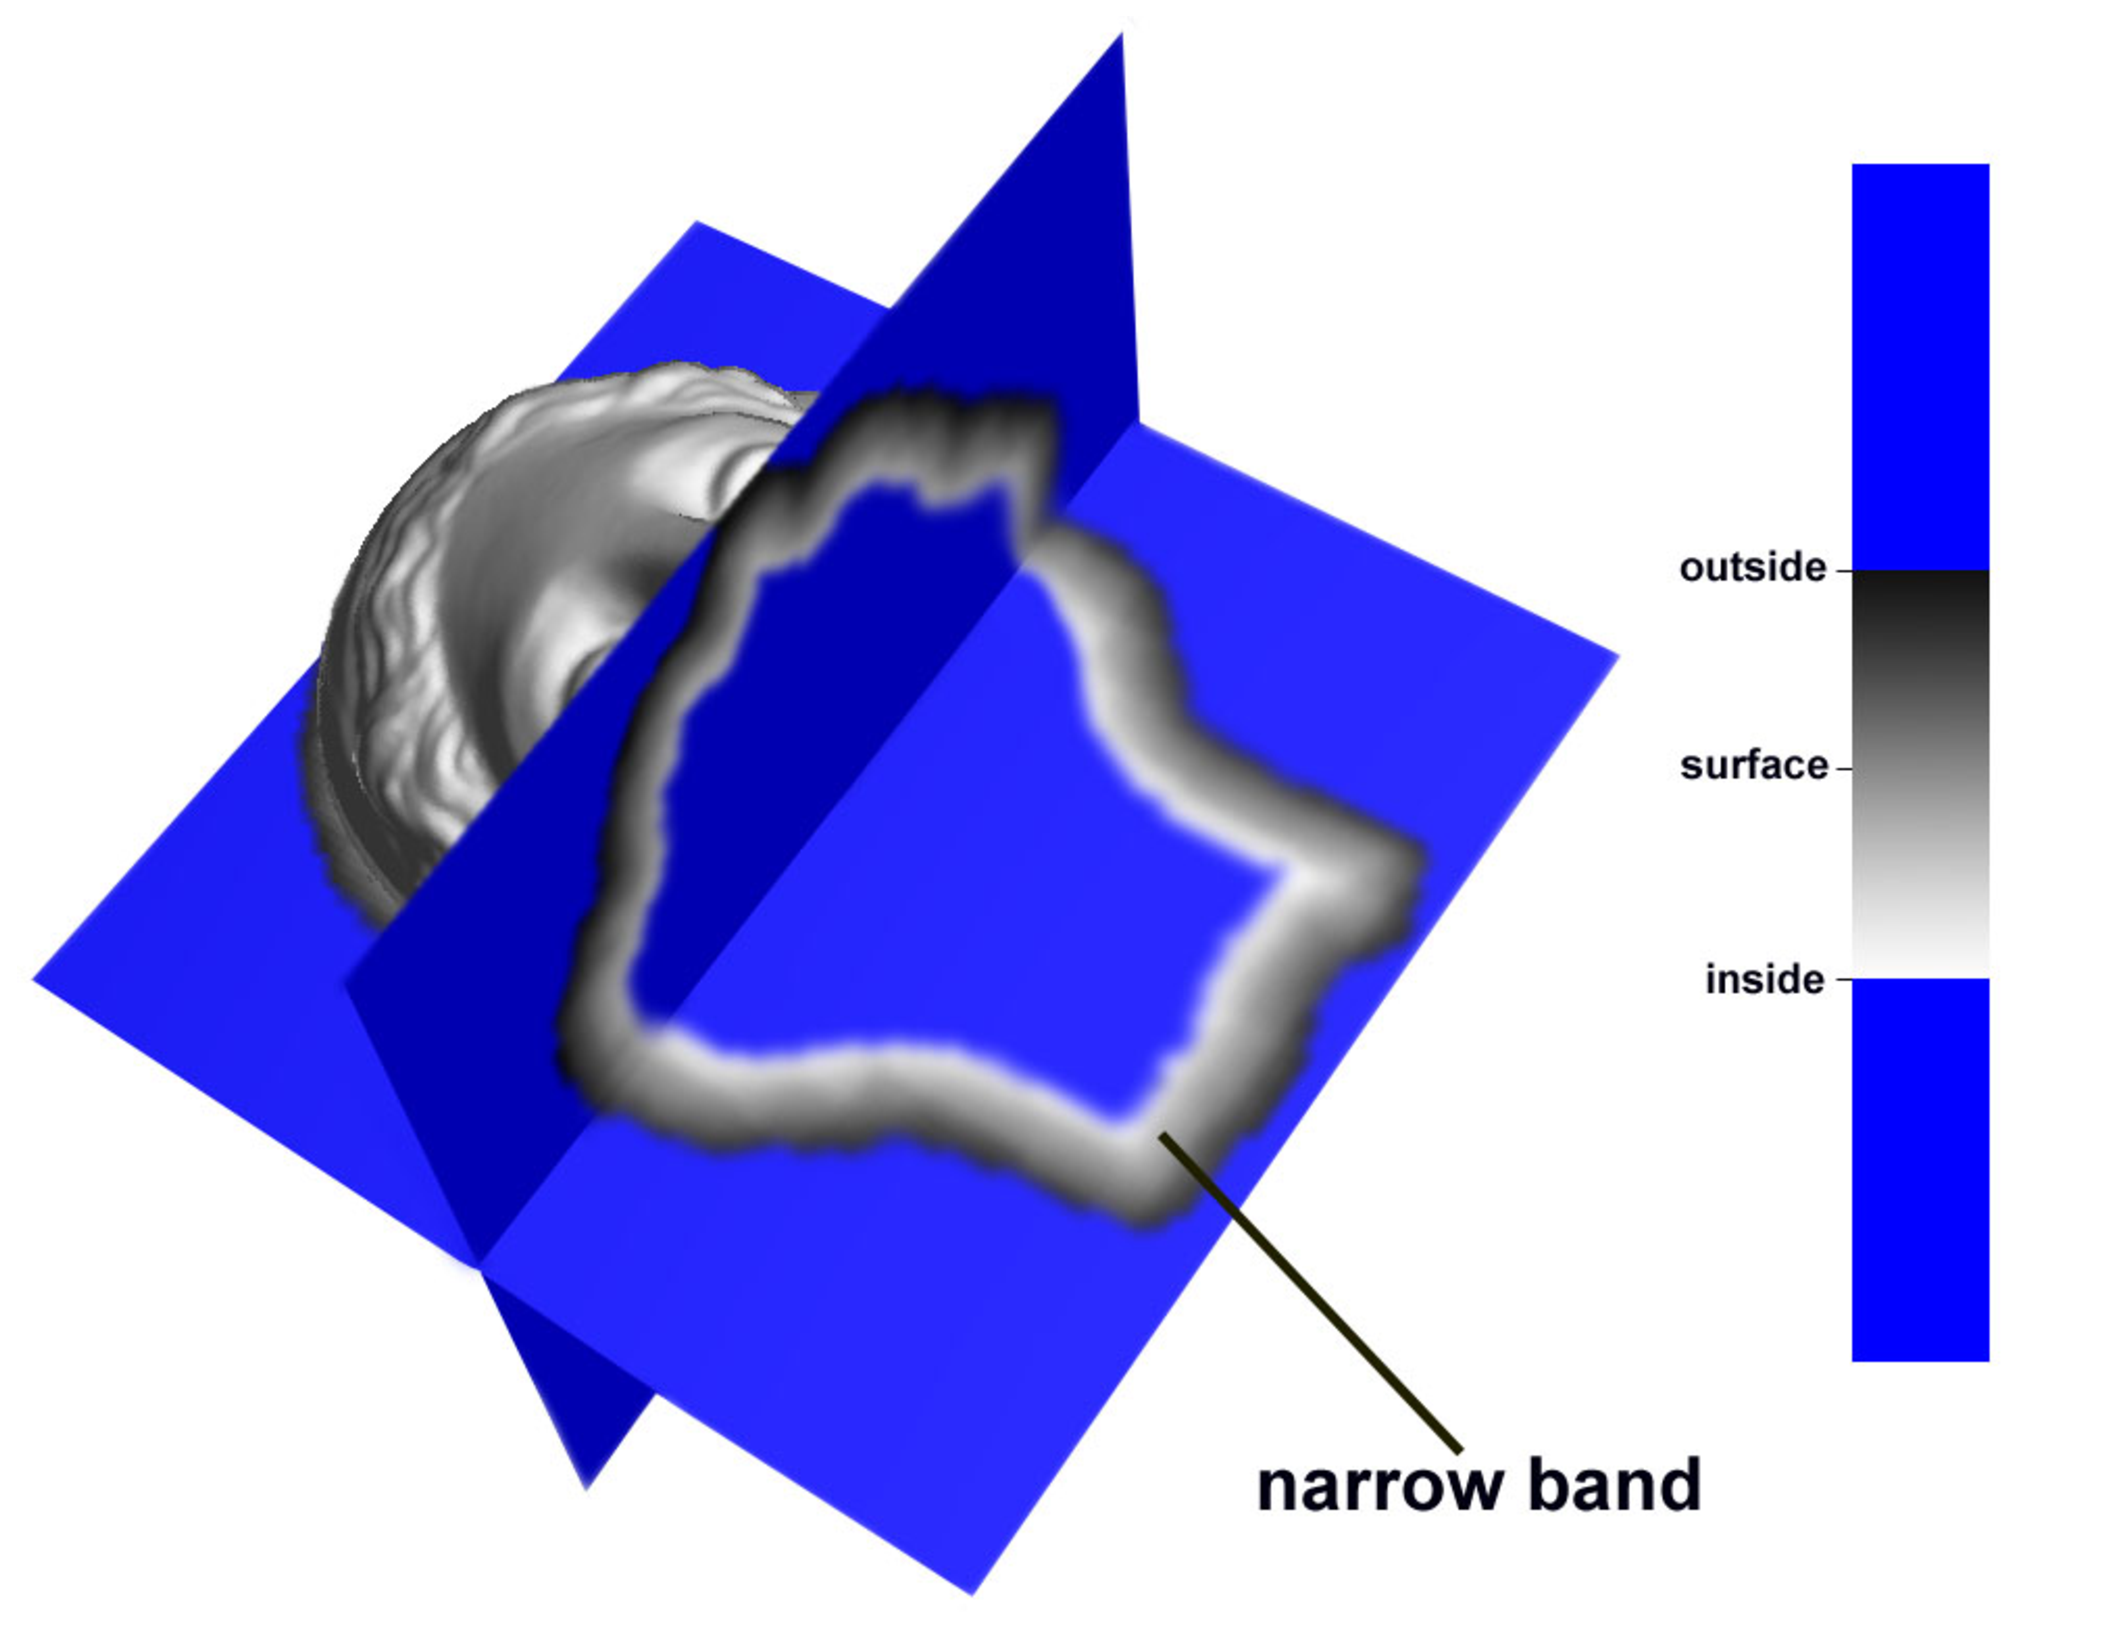
\includegraphics[width=0.487\linewidth]{figures/IgeaNarrowBand}&
    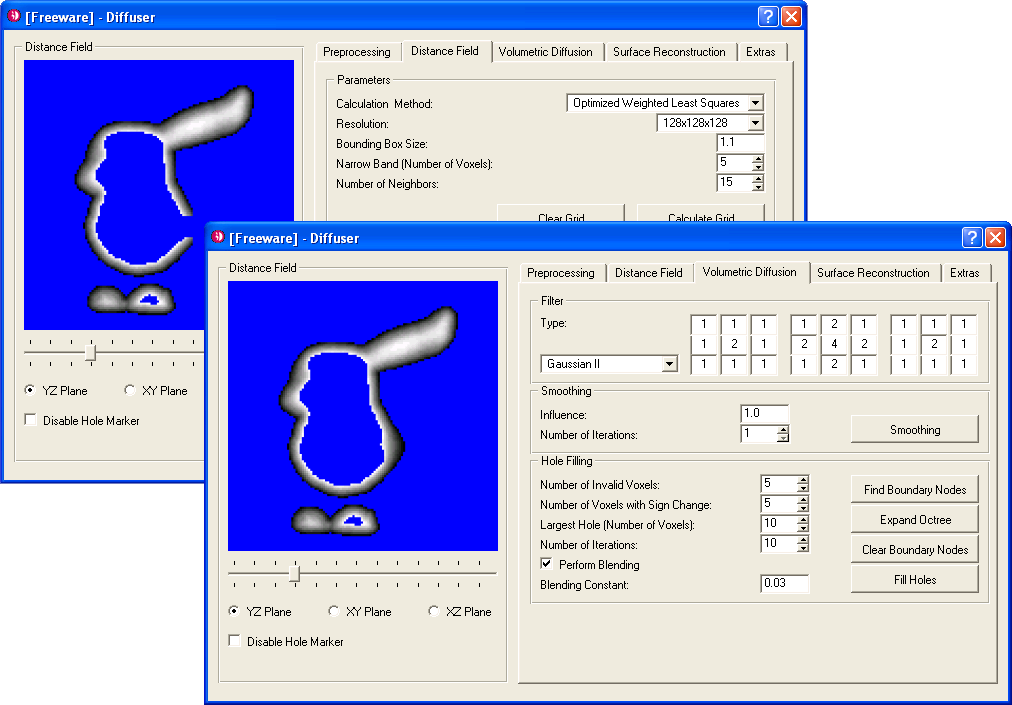
\includegraphics[width=0.487\linewidth]{figures/voldiff_ui}\\
    (a)&(b)\\
    \end{tabular}
    \caption[Volumetric diffusion]{Volumetric diffusion.
    	  \textup{(a)} Slices of the distance volume reveal the narrow band.
			  \textup{(b)} The user interface of the automatic hole filling
        tool allows to fine-tune the algorithm.
        The volumetric representation can be previewed before
        surface reconstruction.%
      \label{fig:voldiff}}
\end{figure}
%
Isn't it?

\begin{figure}[!htb]
	\centering
	\subfigure[Caption first.]{\label{fig:test1}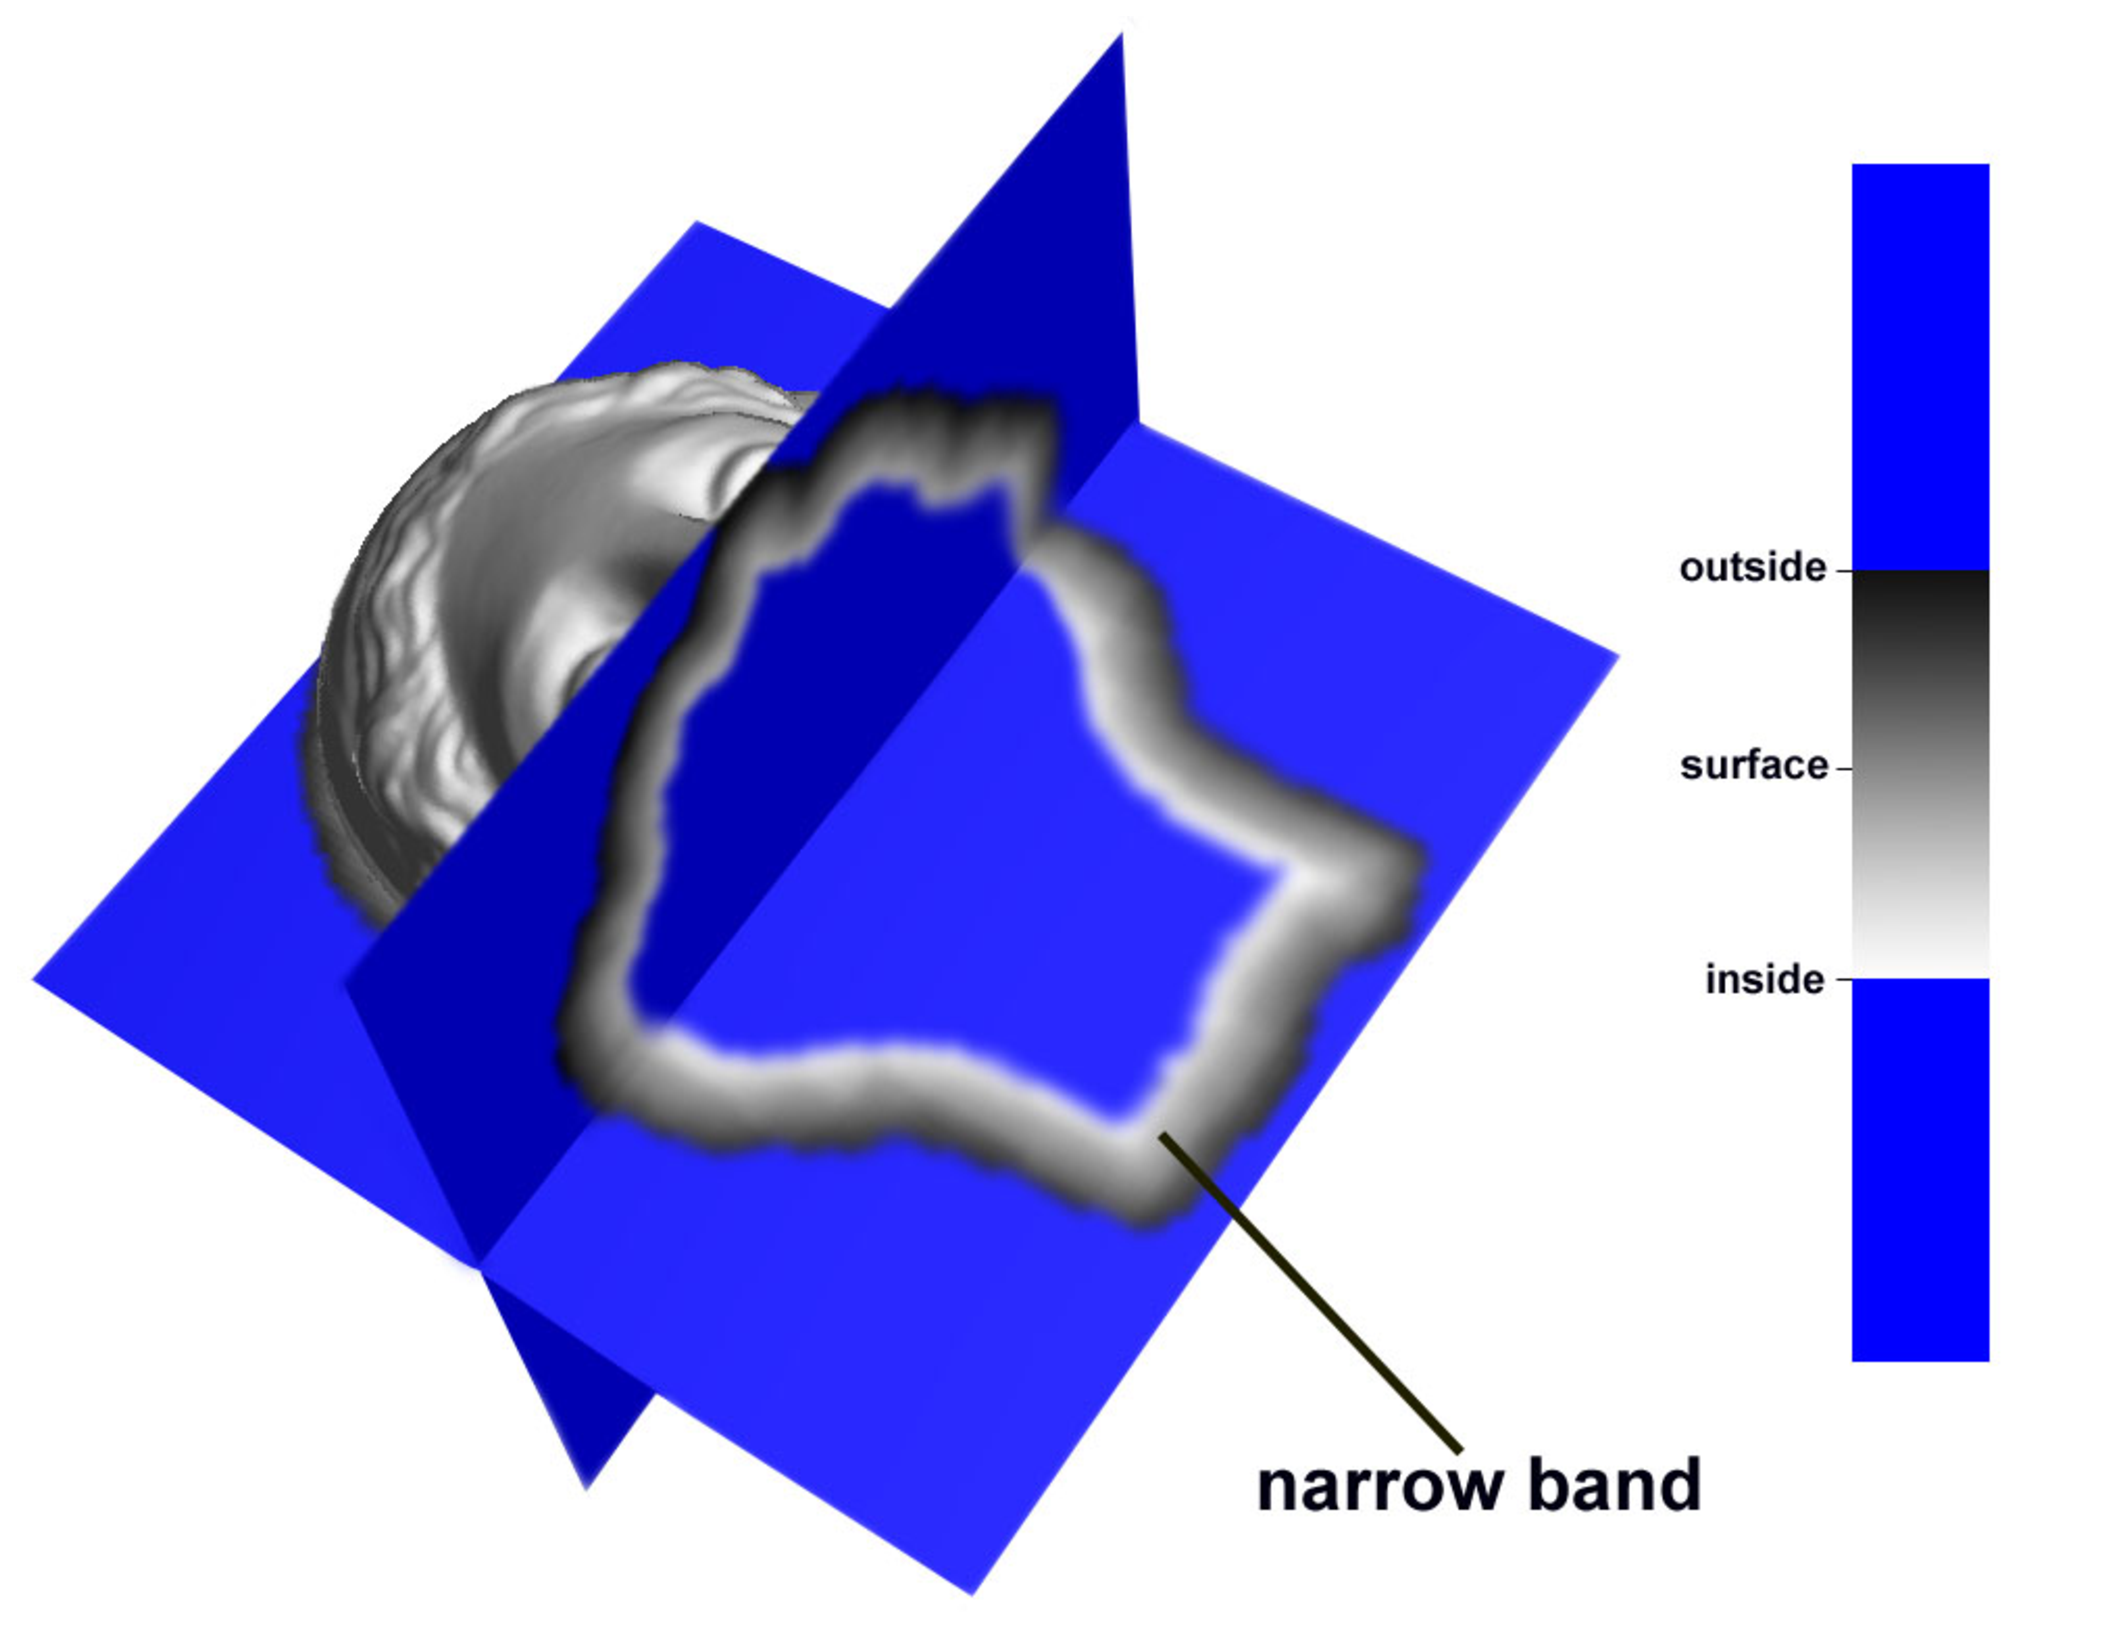
\includegraphics[width=0.3\textwidth]{figures/IgeaNarrowBand}} \hfill
	\subfigure[Caption second.]{\label{fig:test2}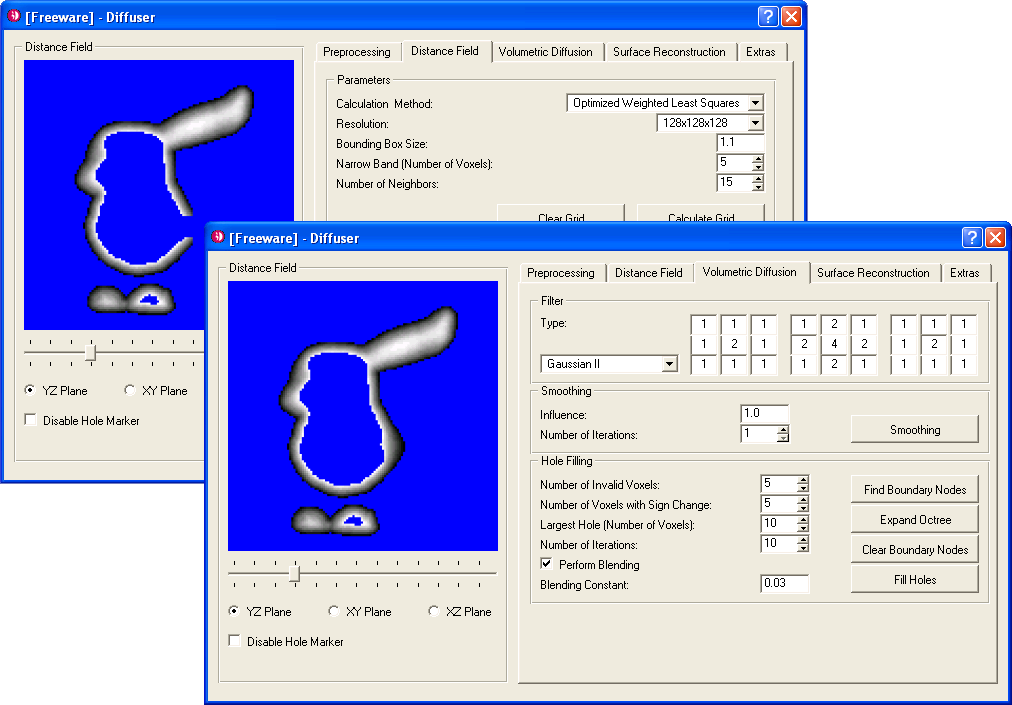
\includegraphics[width=0.3\textwidth]{figures/voldiff_ui}}
	\caption[Caption both]{Caption of both \subref{fig:test1}, \subref{fig:test2}.}
	\label{fig:bothfigures}
\end{figure}


Lorem ipsum dolor sit amet, consectetuer adipiscing elit, sed diam nonummy nibh euismod tincidunt ut laoreet dolore magna aliquam erat volutpat. Ut wisi enim ad minim veniam, quis nostrud exerci tation ullamcorper suscipit lobortis nisl ut aliquip ex ea commodo consequat. Duis autem vel eum iriure dolor in hendrerit in vulputate velit esse molestie consequat, vel illum dolore eu feugiat nulla facilisis at vero et accumsan et iusto odio dignissim qui blandit praesent luptatum zzril delenit augue duis dolore te feugait nulla facilisi. Lorem ipsum dolor sit amet, consectetuer adipiscing elit, sed diam 

\section{Second Section}

Lorem ipsum dolor sit amet, consectetuer adipiscing elit, sed diam nonummy nibh euismod tincidunt ut laoreet dolore magna aliquam erat volutpat. Ut wisi enim ad minim veniam, quis nostrud exerci tation ullamcorper suscipit lobortis nisl ut aliquip ex ea commodo consequat. Duis autem vel eum iriure dolor in hendrerit in vulputate velit esse molestie consequat, vel illum dolore eu feugiat nulla facilisis at vero et accumsan et iusto odio dignissim qui blandit praesent luptatum zzril delenit augue duis dolore te feugait nulla facilisi. Lorem ipsum dolor sit amet, consectetuer adipiscing elit, sed diam nonummy nibh euismod tincidunt ut laoreet dolore magna aliquam erat volutpat. Ut wisi enim ad minim veniam, quis nostrud exerci tation ullamcorper suscipit lobortis nisl ut aliquip ex ea commodo consequat. Duis autem vel eum iriure dolor in hendrerit in vulputate velit esse molestie consequat, vel illum dolore eu feugiat nulla facilisis at vero et accumsan et iusto odio dignissim qui blandit

% \chapter{Conclusion and Outlook}

Lorem ipsum dolor sit amet, consectetuer adipiscing elit, sed diam nonummy nibh euismod tincidunt ut laoreet dolore magna aliquam erat volutpat. Ut wisi enim ad minim veniam, quis nostrud exerci tation ullamcorper suscipit lobortis nisl ut aliquip ex ea commodo consequat. Duis autem vel eum iriure dolor in hendrerit in vulputate velit esse molestie consequat, vel illum dolore eu feugiat nulla facilisis at vero et accumsan et iusto odio dignissim qui blandit praesent luptatum zzril delenit augue duis dolore te feugait nulla facilisi. Lorem ipsum dolor sit amet, consectetuer adipiscing elit, sed diam nonummy nibh euismod tincidunt ut laoreet dolore magna aliquam erat volutpat. Ut wisi enim ad minim veniam, quis nostrud exerci tation ullamcorper suscipit lobortis nisl ut aliquip ex ea commodo consequat. Duis autem vel eum iriure dolor in hendrerit in vulputate velit esse molestie consequat, vel illum dolore eu feugiat nulla facilisis at vero et accumsan et iusto odio dignissim qui blandit

Lorem ipsum dolor sit amet, consectetuer adipiscing elit, sed diam nonummy nibh euismod tincidunt ut laoreet dolore magna aliquam erat volutpat. Ut wisi enim ad minim veniam, quis nostrud exerci tation ullamcorper suscipit lobortis nisl ut aliquip ex ea commodo consequat. Duis autem vel eum iriure dolor in hendrerit in vulputate velit esse molestie consequat, vel illum dolore eu feugiat nulla facilisis at vero et accumsan et iusto odio dignissim qui blandit praesent luptatum zzril delenit augue duis dolore te feugait nulla facilisi. Lorem ipsum dolor sit amet, consectetuer adipiscing elit, sed diam nonummy nibh euismod tincidunt ut laoreet dolore magna aliquam erat volutpat. Ut wisi enim ad minim veniam, quis nostrud exerci tation ullamcorper suscipit lobortis nisl ut aliquip ex ea commodo consequat. Duis autem vel eum iriure dolor in hendrerit in vulputate velit esse molestie consequat, vel illum dolore eu feugiat nulla facilisis at vero et accumsan et iusto odio dignissim qui blandit
Lorem ipsum dolor sit amet, consectetuer adipiscing elit, sed diam nonummy nibh euismod tincidunt ut laoreet dolore magna aliquam erat volutpat. Ut wisi enim ad minim veniam, quis nostrud exerci tation ullamcorper suscipit lobortis nisl ut aliquip ex ea commodo consequat. Duis autem vel eum iriure dolor in hendrerit in vulputate velit esse molestie consequat, vel illum dolore eu feugiat nulla facilisis at vero et accumsan et iusto odio dignissim qui blandit praesent luptatum zzril delenit augue duis dolore te feugait nulla facilisi. Lorem ipsum dolor sit amet, consectetuer adipiscing elit, sed diam nonummy nibh euismod tincidunt ut laoreet dolore magna aliquam erat volutpat. Ut wisi enim ad minim veniam, quis nostrud exerci tation ullamcorper suscipit lobortis nisl ut aliquip ex ea commodo consequat. Duis autem vel eum iriure dolor in hendrerit in vulputate velit esse molestie consequat, vel illum dolore eu feugiat nulla facilisis at vero et accumsan et iusto odio dignissim qui blandit

Lorem ipsum dolor sit amet, consectetuer adipiscing elit, sed diam nonummy nibh euismod tincidunt ut laoreet dolore magna aliquam erat volutpat. Ut wisi enim ad minim veniam, quis nostrud exerci tation ullamcorper suscipit lobortis nisl ut aliquip ex ea commodo consequat. Duis autem vel eum iriure dolor in hendrerit in vulputate velit esse molestie consequat, vel illum dolore eu feugiat nulla facilisis at vero et accumsan et iusto odio dignissim qui blandit praesent luptatum zzril delenit augue duis dolore te feugait nulla facilisi. Lorem ipsum dolor sit amet, consectetuer adipiscing elit, sed diam nonummy nibh euismod tincidunt ut laoreet dolore magna aliquam erat volutpat. Ut wisi enim ad minim veniam, quis nostrud exerci tation ullamcorper suscipit lobortis nisl ut aliquip ex ea commodo consequat. Duis autem vel eum iriure dolor in hendrerit in vulputate velit esse molestie consequat, vel illum dolore eu feugiat nulla facilisis at vero et accumsan et iusto odio dignissim qui blandit



% ---- END MAIN PART ----


% \appendix
\clearpage
\renewcommand*{\chapterpagestyle}{myappendixpagestyle}

% \chapter{Information For The Few}

Nein, meine Texte les ich nicht, so nicht, stöhnte Oxmox. Er war mit Franklin, Rockwell und dem halbtaxgrauen Panther Weidemann in Memphis (Heartbreak Hotel) zugange. Sie warteten auf die fette Gill, um bei der Bank of Helvetica die Kapitälchen in Kapital umzuwandeln. Oxmox liess nicht locker. Ich fleh euch an, rettet meine Copy, gebt meinem Body nochn Durchschuss! Kein Problem, erbarmte sich Old Face Baskerville, streichelte seinen Hund, zog seine einspaltige Poppl, legte an und traf! (Zeidank nichts Ernstes --- nurn bisschen Fraktur.) Oxmox: Danke, ist jetzt mit Abstand besser. Derweil jumpte der Fox leise over the Buhl, die sich mal wieder immerdar wie jedes Jahr gesellte. Diesmal war Guaredisch ihr Erwählter, weil seine Laufweite einem vollgetankten Bodoni entsprach und seine ungezügelte Unterlänge ihre Serifen so serafisch streifte, dass sie trotz Techtelmechtelei die magere Futura, jene zuverlässige und gern eingesetzte Langstreckenläuferin, rechtsbündig überholen konnten.

\section{Foo Bar Baz}

Nein, meine Texte les ich nicht, so nicht, stöhnte Oxmox. Er war mit Franklin, Rockwell und dem halbtaxgrauen Panther Weidemann in Memphis (Heartbreak Hotel) zugange. Sie warteten auf die fette Gill, um bei der Bank of Helvetica die Kapitälchen in Kapital umzuwandeln. Oxmox liess nicht locker. Ich fleh euch an, rettet meine Copy, gebt meinem Body nochn Durchschuss! Kein Problem, erbarmte sich Old Face Baskerville, streichelte seinen Hund, zog seine einspaltige Poppl, legte an und traf! (Zeidank nichts Ernstes --- nurn bisschen Fraktur.) Oxmox: Danke, ist jetzt mit Abstand besser. Derweil jumpte der Fox leise over the Buhl, die sich mal wieder immerdar wie jedes Jahr gesellte. Diesmal war Guaredisch ihr Erwählter, weil seine Laufweite einem vollgetankten Bodoni entsprach und seine ungezügelte Unterlänge ihre Serifen so serafisch streifte, dass sie trotz Techtelmechtelei die magere Futura, jene zuverlässige und gern eingesetzte Langstreckenläuferin, rechtsbündig überholen konnten.

\section{Barontes}

Nein, meine Texte les ich nicht, so nicht, stöhnte Oxmox. Er war mit Franklin, Rockwell und dem halbtaxgrauen Panther Weidemann in Memphis (Heartbreak Hotel) zugange. Sie warteten auf die fette Gill, um bei der Bank of Helvetica die Kapitälchen in Kapital umzuwandeln. Oxmox liess nicht locker. Ich fleh euch an, rettet meine Copy, gebt meinem Body nochn Durchschuss! Kein Problem, erbarmte sich Old Face Baskerville, streichelte seinen Hund, zog seine einspaltige Poppl, legte an und traf! (Zeidank nichts Ernstes --- nurn bisschen Fraktur.) Oxmox: Danke, ist jetzt mit Abstand besser. Derweil jumpte der Fox leise over the Buhl, die sich mal wieder immerdar wie jedes Jahr gesellte. Diesmal war Guaredisch ihr Erwählter, weil seine Laufweite einem vollgetankten Bodoni entsprach und seine ungezügelte Unterlänge ihre Serifen so serafisch streifte, dass sie trotz Techtelmechtelei die magere Futura, jene zuverlässige und gern eingesetzte Langstreckenläuferin, rechtsbündig überholen konnten.


\section{A Long Table with Booktabs}


{\scriptsize
\begin{longtable}{clccccccc}
\caption[wordlist]{A sample list of words.}\\
\toprule
ID & Word & Word Length & WD & ETL & PTL &  WDplus \\
\midrule
\endfirsthead
\caption[]{(Continued)}\\
\toprule
ID & Word & Word Length & WD & ETL & PTL &  WDplus \\
\midrule
\endhead
\midrule
\multicolumn{9}{c}{continued on next page}\\
\bottomrule
\endfoot
%\bottomrule
\endlastfoot
\hline
1 & Eis & 3 & 4 & 0.42 & 1.83 & 0.19 \\ \hline
2 & Mai & 3 & 5 & 0.49 & 1.92 & 0.19 \\ \hline
3 & Art & 3 & 5 & 0.27 & 1.67 & 0.14 \\ \hline
4 & Uhr & 3 & 5 & 0.57 & 1.87 & 0.36 \\ \hline
5 & Rat & 3 & 5 & 0.36 & 1.71 & 0.14 \\ \hline
6 & weit & 4 & 6 & 0.21 & 1.65 & 0.25 \\ \hline
7 & eins & 4 & 6 & 0.38 & 1.79 & 0.26 \\ \hline
8 & Wort & 4 & 6 & 0.30 & 1.62 & 0.20 \\ \hline
9 & Wolf & 4 & 6 & 0.18 & 1.54 & 0.19 \\ \hline
10 & Wald & 4 & 6 & 0.31 & 1.63 & 0.19 \\ \hline
11 & Amt & 3 & 6 & 0.30 & 1.67 & 0.14 \\ \hline
12 & Wahl & 4 & 7 & 0.36 & 1.77 & 0.42 \\ \hline
13 & Volk & 4 & 7 & 0.45 & 1.81 & 0.20 \\ \hline
14 & Ziel & 4 & 7 & 0.48 & 1.78 & 0.42 \\ \hline
15 & vier & 4 & 7 & 0.38 & 1.81 & 0.42 \\ \hline
16 & Kreis & 5 & 7 & 0.26 & 1.62 & 0.33 \\ \hline
17 & Preis & 5 & 7 & 0.28 & 1.51 & 0.33 \\ \hline
18 & Re-de & 4 & 7 & 0.22 & 1.56 & 0.33 \\ \hline
19 & Saal & 4 & 7 & 0.75 & 2.10 & 0.43 \\ \hline
20 & voll & 4 & 7 & 0.48 & 1.82 & 0.24 \\ \hline
21 & weiss & 5 & 7 & 0.21 & 1.59 & 0.36 \\ \hline
22 & Är-ger & 5 & 7 & 1.16 & 2.69 & 0.59 \\ \hline
23 & bald & 4 & 7 & 0.18 & 1.56 & 0.19 \\ \hline
24 & hier & 4 & 7 & 0.40 & 1.70 & 0.43 \\ \hline
25 & neun & 4 & 7 & 0.17 & 1.52 & 0.26 \\ \hline
26 & sehr & 4 & 7 & 0.36 & 1.85 & 0.43 \\ \hline
27 & Jahr & 4 & 7 & 0.50 & 1.82 & 0.43 \\ \hline
28 & Gold & 4 & 7 & 0.04 & 1.35 & 0.20 \\ \hline
29 & Tä-ter & 5 & 8 & 0.15 & 1.39 & 0.59 \\ \hline
30 & Tei-le & 5 & 8 & 0.30 & 1.71 & 0.46 \\ \hline
31 & Na-tur & 5 & 8 & 0.18 & 1.59 & 0.41 \\ \hline
32 & Feu-er & 5 & 8 & 0.30 & 1.71 & 0.45 \\ \hline
33 & Rol-le & 5 & 8 & 0.15 & 1.46 & 0.45 \\ \hline
34 & Rock & 4 & 8 & 0.29 & 1.68 & 0.25 \\ \hline
35 & Spass & 5 & 8 & 0.28 & 1.64 & 0.32 \\ \hline
36 & Gäs-te & 5 & 8 & 0.49 & 1.75 & 0.66 \\ \hline
37 & En-de & 4 & 8 & 0.36 & 1.72 & 0.33 \\ \hline
38 & Kunst & 5 & 8 & 0.26 & 1.59 & 0.35 \\ \hline
39 & Li-nie & 5 & 8 & 0.45 & 1.88 & 0.63 \\ \hline
40 & Bäu-me & 5 & 8 & 0.48 & 1.92 & 0.45 \\ \hline
41 & Büh-ne & 5 & 9 & 0.94 & 2.48 & 0.62 \\ \hline
42 & Bahn & 4 & 9 & 0.21 & 1.62 & 0.42 \\ \hline
43 & Bür-ger & 6 & 9 & 0.38 & 1.70 & 0.65 \\ \hline
44 & Druck & 5 & 9 & 0.60 & 2.03 & 0.31 \\ \hline
45 & zehn & 4 & 9 & 0.41 & 1.84 & 0.42 \\ \hline
46 & Va-ter & 5 & 9 & 0.36 & 1.78 & 0.40 \\ \hline
47 & Angst & 5 & 9 & 0.29 & 1.56 & 0.35 \\ \hline
48 & lei-der & 6 & 9 & 0.13 & 1.47 & 0.52 \\ \hline
49 & häu-fig & 6 & 9 & 0.82 & 2.31 & 0.52 \\ \hline
50 & le-ben & 5 & 9 & 0.38 & 1.85 & 0.40 \\ \hline
51 & aus-ser & 6 & 9 & 1.20 & 2.26 & 0.57 \\ \hline
52 & be-vor & 5 & 9 & 1.28 & 2.75 & 0.39 \\ \hline
53 & Kai-ser & 6 & 9 & 0.92 & 2.37 & 0.53 \\ \hline
54 & Markt & 5 & 9 & 0.23 & 1.58 & 0.28 \\ \hline
55 & Os-ten & 5 & 9 & 0.21 & 1.54 & 0.48 \\ \hline
56 & Krieg & 5 & 9 & 0.33 & 1.67 & 0.50 \\ \hline
57 & Mann & 4 & 9 & 0.31 & 1.47 & 0.25 \\ \hline
58 & Hal-le & 5 & 9 & 0.24 & 1.65 & 0.45 \\ \hline
59 & heu-te & 5 & 9 & 0.44 & 1.87 & 0.46 \\ \hline
60 & in-nen & 5 & 10 & 0.36 & 1.80 & 0.45 \\ \hline
61 & Na-men & 5 & 10 & 0.28 & 1.72 & 0.41 \\ \hline
62 & jetzt & 5 & 10 & 0.70 & 2.07 & 0.32 \\ \hline
63 & kei-ner & 6 & 10 & 0.28 & 1.62 & 0.53 \\ \hline
64 & Schu-le & 6 & 10 & 1.02 & 2.12 & 0.48 \\ \hline
65 & Ar-beit & 6 & 10 & 0.34 & 1.70 & 0.52 \\ \hline
66 & An-teil & 6 & 10 & 0.27 & 1.63 & 0.53 \\ \hline
67 & di-rekt & 6 & 10 & 0.67 & 2.04 & 0.47 \\ \hline
68 & vor-her & 6 & 10 & 0.78 & 2.25 & 0.47 \\ \hline
69 & wol-len & 6 & 10 & 0.44 & 1.85 & 0.51 \\ \hline
70 & Kampf & 5 & 10 & 0.70 & 1.96 & 0.27 \\ \hline
71 & än-dern & 6 & 10 & 1.18 & 2.62 & 0.65 \\ \hline
72 & lau-fen & 6 & 10 & 0.21 & 1.64 & 0.52 \\ \hline
73 & Eu-ro-pa & 6 & 10 & 0.23 & 1.53 & 0.66 \\ \hline
74 & statt & 5 & 10 & 1.61 & 2.86 & 0.39 \\ \hline
75 & Wes-ten & 6 & 10 & 0.29 & 1.60 & 0.54 \\
\bottomrule
\label{tab:wordlist}
\end{longtable}
}

\clearpage
\renewcommand*{\chapterpagestyle}{empty}

%\nocite{*}
\addcontentsline{toc}{chapter}{Bibliography}
\bibliography{graphics}

\end{document}
